\cotefile{33}
\scanpage{2}
Nous prendrons comme prétexte la théorie des fonctions $L$ pour développer plus avant le formalisme de la cohomologie étale. Trois parties

a) Continuer l'étude \inserted{de la coh. étale} avec des coefficients de torsion, en développant en particulier, dans ce cadre, \deleted{\unsure{plus}} \deleted{\unsure{axiomatique}} \unsure{bien avant} le formalisme de dualité, \deleted{\unsure{donnant}} donnant des formules de Künneth et de Lefschetz.

b) Étendre le formalisme : des coefficients \uline{$l$-adiques}.

c) Appliquer les résultats au formalisme des fonctions $L$.

1°) \uline{Site étale} de $X$ ;
\[
\begin{array}{ll}
X_{\mathrm{ét}} : & \text{catégorie}\\
&\text{familles couvrantes}\\
&\text{faisceaux}\\
&\text{faisceaux abéliens}\\
&\text{cohomologie}
\end{array}
\]

2°) \uline{Exemple} $X-\unsure{\operatorname{Spec}k|\operatorname{Spm}k}$,
\[
X_{\mathrm{ét}}\simeq\widetilde X_{\mathrm{ét}}\simeq\operatorname{Ens}(\pi)
\qquad \pi=\operatorname{Gal}(\bar k/k)
\]

3°) $f:X\longrightarrow Y$ \unsure{définit}
\[
X_{\mathrm{ét}}-Y_{\mathrm{ét}}
\]
\[
\left\{\begin{aligned}
f^* &:Y_{\mathrm{ét}}\longrightarrow X_{\mathrm{ét}}\\
&:\widetilde Y_{\mathrm{ét}}\longrightarrow\widetilde X_{\mathrm{ét}}
\end{aligned}\right.
\]
\[
f_* :\widetilde X_{\mathrm{ét}}\longrightarrow\widetilde Y_{\mathrm{ét}}
\]
\margin{commute aux $\unsure{\varinjlim}$ \unsure{quelc.} et aux $\unsure{\varprojlim}$ finies}
\margin{commute aux $\unsure{\varprojlim}$ \unsure{quelc.}}
\mspage{1}
\scanpage{3}
\diagram{\begin{tikzcd}[column sep=small]
\unsure{k'}\arrow[ddr,no head,bend right=18]\arrow[rr,no head,bend left=45] & |[draw,ellipse]|\unsure{X}\arrow[dd] & \unsure{X_K}\arrow[l,Rightarrow]\arrow[dd,no head]\arrow[dd,no head,bend left=18]\\
&&\\
&\unsure{k}&\unsure{K}\arrow[l,no head]
\end{tikzcd}}

\figure{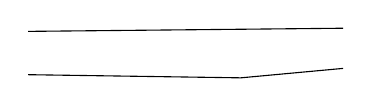
\begin{tikzpicture}
\draw (0,0)--(4,0.04);\draw (0,-.55)--(2.7,-.59)--(4,-.47);
\end{tikzpicture}}

\diagram{\begin{tikzcd}[column sep=small]
\unsure{Y}\arrow[r]\arrow[dr,no head]&X\arrow[d,no head]&&\unsure{Y'}\arrow[r]\arrow[dr,no head]&X'\arrow[d,no head]\\
&\unsure{k}\arrow[rrr,no head,"{\textcircled{\scriptsize\unsure{$\varphi$}}}"']&&{}\arrow[d]&\unsure{k'}\\
&&&{}&
\end{tikzcd}}

\diagram{\begin{tikzcd}
\unsure{Y}\arrow[d,"f"'] & \unsure{Y'}\arrow[l,"h"']\arrow[d,"f'"] & \unsure{V'}\\
X & X'\arrow[l,"g"',very thick]\arrow[d,no head,bend left=25] &\\
\unsure{g(U\prime)} & \unsure{U'\ne\varnothing}&
\end{tikzcd}}
\figure{\begin{tikzpicture}
\draw (0,0) .. controls (1,0.9) and (3,0.9) .. (4,0);
\draw (0,-.2) .. controls (-.3,-1) and (-.3,-2) .. (0,-2.5);
\end{tikzpicture}}

\diagram{\begin{tikzcd}
X'\arrow[r]\arrow[dr] &X\arrow[d,no head]\\
\unsure{\ne\varnothing}&\unsure{k}
\end{tikzcd}}

\diagram{\begin{tikzcd}
X\arrow[d,no head]&\\
\unsure{k}\arrow[r,no head]&Y
\end{tikzcd}}

\[
\unsure{A}\ -
\qquad
\begin{array}{c}
M\unsure{\subset|c}L\\
\times\,\unsure{M'U}
\end{array}
\]
\mspage{2}
\scanpage{4}
transitivité -{}-{}-
\[R^i f_*\]
\uline{Suite spectrale de Leray}
\margin{....}

4°) Foncteurs fibres

Soit $\xi$ un pt géométrique de $X$
\[
\xi\xrightarrow{i}X,\quad \text{d'où foncteur fibre}
\]
\[
i^*:\widetilde X_{\mathrm{ét}}\longrightarrow\widetilde\xi_{\mathrm{ét}}\simeq(\operatorname{Ens})
\]
La famille des foncteurs fibres est \uline{conservative} : $u:F-G$ est un isom ssi les $u_{\bar x}:F_{\bar x}-G_{\bar x}$ le sont pour tt $x\in X$ d'où les cor. habituels.
\[
F_\xi=\underset{\substack{X'\text{ étale sur}\\X\text{ et pointé}\\\text{par }\xi}}{\unsure{\varinjlim}}F(X')
\]

5°) Localisation stricte
\diagram{\begin{tikzcd}
X'\arrow[d]&\xi\arrow[l]\arrow[dl]\\
X&
\end{tikzcd}}
\[
\underline{\mathcal O}_{X,\xi}\deleted{\unsure{\xi_X}}
=\underset{\substack{X'\text{ étale sur}\\X\text{ et }\xi\text{-pointé}}}{\underset{\longleftrightarrow}{\operatorname{Lim}}}
\Gamma(X',\mathcal O_{X'})
\]
\margin{anneaux stricts locaux ou \unsure{strict.t local} i.e.\ \deleted{\unsure{hensélien et}} hensélien et à corps rés. sép. clos}
\[
\bar X^{\unsure{\xi}}=\operatorname{Spec}\mathcal O_{X,\xi}
\]
\[
F_\xi=\Gamma(\bar X,\unsure{\widetilde F}_{\bar X})
\]

6°) Application aux fibres des $R^qf_*(F)$, pour $f$ qu. cpt. et qu. sép.

\margin{\uline{NB} 5° et 6° \unsure{n'a} pas vraiment d'analogue complet dans le cas des espaces top. ordinaires .....}
\figure{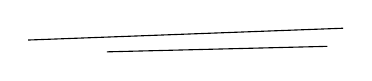
\begin{tikzpicture}\draw (0,0)--(4,.15);\draw (1,-.15)--(3.8,-.08);\end{tikzpicture}}

7°) \uuline{Théorème fondamental} Soit $f:X-Y$ un morphisme propre, $F$ faisceau \uline{de torsion} sur $X$, alors la formation des $R^{\unsure{i|q}}f_*(F)$
\mspage{3}
\scanpage{5}
\margin{....}
\begin{center}- 180 -\end{center}
\margin{n° 391}

Alors, (\S\ 1, n° 3, prop. 8), on aurait $\displaystyle\sum_{k\ne i}q_{ik}^2\geq\frac14+(\frac{\sqrt3}{2})^2=1$, ce qui contredit le lemme 1.

COROLLAIRE 4.- \uline{Un sommet ne peut appartenir à deux arêtes distinctes d'ordre} $\geq4$.

En effet, (\S\ 1, n° 3, prop. 8), on a $(\frac{\sqrt2}{2})^2+(\frac{\sqrt2}{2})^2=1$.

Soit $\{i,j\}$ une arête de $X$ ; soit $\underline M'=(m'_{hk})$, $(1\leq h\leq\ell,\ 1\leq k\leq\ell,\ h\ne j,\ k\ne j)$, la matrice d'ordre $\ell-1$ définie par $m'_{hk}=m_{hk}$ si $h\ne i$ ou $k\ne i$, $m'_{ik}=m'_{ki}=m_{ik}+m_{jk}$ pour tout $k$ distinct de $i$ et de $j$, $m'_{ii}=m_{ii}=1$. On dit que le schéma de Coxeter $X'$ de $\underline M'$ s'obtient à partir de $X$ \uline{identifiant} $j$ \uline{à} $i$. Les arêtes de $X'$ sont donc les ensembles $\{i,k\}$, $(k\ne j)$, qui sont des arêtes de $X$, les ensembles $\{i,k'\}$, $(k'\ne j)$, tels que $\{j,k'\}$ soit une arête de $X$, et les arêtes $\{k,k'\}$ de $X$ liant des sommets distincts de $i$ et de $j$. Si $k$ est distinct de $i$ et de $j$, on notera que $\{i,k\}$ et $\{j,k\}$ ne peuvent tous deux être des arêtes de $X$, sans quoi elles formeraient avec $\{i,j\}$ un circuit dans $X$ ; on en conclut que si $k$ est \uline{point de ramification} dans $X$, il l'est encore dans $X'$.

LEMME 2.- \uline{Si l'arête} $\{i,j\}$ \uline{est d'ordre} 3, $G(\underline M')$ \uline{est un groupe fini}.

Notons en effet que si $k$ est distinct de $i$ et de $j$, on ne peut avoir \uline{à la fois} $m_{ik}\geq3$ et $m_{jk}\geq3$, sans quoi les arêtes $\{i,j\}$, $\{j,k\}$, $\{k,i\}$ formeraient un circuit dans $X$. Si on pose $q'_{hk}=-\cos(\pi/m'_{hk})$, $(h,k\text{ distincts de }j)$, on a donc $q'_{ik}=q_{ik}+q_{jk}$ pour $k$ distinct de $i$ et de $j$ ; comme $q_{ii}=q_{jj}=1$ et $q_{ij}=-\frac12$ par hypothèse, on voit que la forme quadratique $B_{\underline M'}$ est telle que pour $\displaystyle x=\sum_{k\ne j}\xi_ke_k$, $B_{\underline M'}(x,x)$ soit égal au nombre obtenu en remplaçant $\xi_j$ par $\xi_i$ dans $q(\xi_1,\ldots,\xi_\ell)$ ; on a donc $B_{\underline M'}(x,x)>0$ par hypothèse si $x\ne0$.
\mspage{4}
\scanpage{6}
\mspage{5}
commute à tt changement de base $Y'-Y$.

\uline{NB} Vrai sans hyp. de propreté si $Y'\to Y$ est \uline{lisse}, $f$ qu. cpt. qu. sép., et $F$ premier aux car. rés. de $Y$.

\deleted{\unsure{8°)} \uline{Ex} Morphisme fini $R^qf_*(F)=0\quad q\ne0$}

\figure{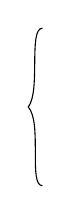
\begin{tikzpicture}\draw (.18,1) .. controls (0,1) and (.16,.2) .. (0,0) .. controls (.18,-.2) and (0,-1) .. (.18,-1);\end{tikzpicture}}
\uline{Ex}
\[
R^qf_*(F)_{\bar y}\simeq H^q(X_{\bar y},F_{\bar y})
\]
\uline{Ex.} $X$ \inserted{prop.} sur $k$ sép. clos, $k'$ ext. sép. clos de $k$, d'où $X'=X_{k'}$, $F'=F_{X'}$, et $H^i(X,F)\simeq H^i(X',F')$.

\uline{NB} Vrai sans hyp. de propreté si $F$ de torsion \unsure{première} à \deleted{\unsure{la car.}} $\operatorname{car} k$.

8°) \uline{Comparaison avec la cohomologie classique}

$X$ \unsure{préschéma} loc. alg. sur $\mathbf C$, alors pour tt $F$ faisceau de torsion sur $X$,
\[
H^q(X,F)\longrightarrow H^q(X^{\mathrm{tr}},F^{\mathrm{tr}})
\]
est un \uline{isomorphisme}. Résultat analogue pour un morphisme $f:X\longrightarrow Y$, si $f$ est \deleted{propre} \uline{de type fini}.

\margin{Utilise en plus résolution \unsure{sing.} \unsure{si on fait|sauf} \deleted{\unsure{avec}} l'hyp de propreté.}

\margin{\uline{Gaga} plus complet : OK. pour \deleted{\unsure{Hom}} \unsure{Ét} \unsure{les} faisceaux de torsion : équivalence de catégories des faisceaux constructibles algébriques et faisceaux constructibles analytiques qui sont \uline{de torsion}. \unsure{à rédiger} .....}

\deleted{\uline{Remarque} Soit $X$ un schéma propre sur un \unsure{anneau} analytique \inserted{$A=\mathcal O_{Y,y}$} sur $\mathbf C$, i.e. $Y$ un \unsure{espace} analytique sur $\mathbf C$. Alors $X$ ``provient'' d'un \unsure{schéma} analytique $X'$ \uline{propre} au dessus d'un voisinage ouvert $Y'$ de $Y$. \deleted{\unsure{A pour un faisceau}} tt faisceau \inserted{de torsion} constr. $F'$ sur $X'$ ``induit'' un \deleted{\unsure{faisceau}} constr. $F$ sur $X$.}
\scanpage{7}
\begin{center}- 179 -\end{center}
\margin{n° 391}

conséquences sur les $m_{ij}$ qui permettront de dresser la liste de toutes les possibilités pour les schémas de Coxeter correspondants ; il restera ensuite à voir que ces possibilités sont effectivement réalisées, c'est-à-dire que les groupes correspondants $G(\underline M)$ sont \uline{finis}, (ou encore que la forme $q$ est positive non dégénérée).

LEMME 1.- \uline{Pour tout} $i$, \uline{on a} $\displaystyle\sum_{j\ne i}q_{ij}^2<1$.

On peut se borner à ne considérer que les indices $j$ pour lesquels $q_{ij}\ne0$, c'est-à-dire ceux qui sont liés à $i$ dans $X$. Si $j$, $j'$ sont deux de ces indices distincts, $\{j,j'\}$ n'est pas une arête, sinon $\{i,j\}$, $\{j,j'\}$ et $\{j',i\}$ formeraient un circuit dans $X$ ; donc $e_j$ et $e_{j'}$ sont \uline{orthogonaux}, et le lemme résulte du fait que, dans $E$, la distance $d$ de $e_i$ au sous-espace vectoriel $F$ engendré par les $e_j$, ($j$ lié à $i$), est donnée par $\displaystyle d^2=1-\sum_j(e_i\mid e_j)^2=1-\sum_{j\ne i}q_{ij}^2$ en vertu du th. de Pythagore, les $e_j$ formant une base orthonormale de $F$.

COROLLAIRE 1.- \uline{Un sommet de} $X$ \uline{ne peut appartenir qu'à} 3 \uline{arêtes au plus}.

En effet, si $i$ est lié à $h$ autres sommets, les relations $q_{ij}^2\geq1/4$ pour ces sommets $j$ entraînent $h/4<1$ par le lemme 1, donc $h\leq3$.

COROLLAIRE 2.- \uline{Si} $i$ \uline{appartient à} 3 \uline{arêtes}, \uline{ces arêtes sont d'ordre} 3.

Comme $\cos(\pi/m)\geq\sqrt2/2$ pour $m\geq4$, (\S\ 1, n° 3, prop. 8), on aurait en effet, dans le cas contraire, $\displaystyle\sum_{j\ne i}q_{ij}^2\geq\frac14+\frac14+\frac12=1$, ce qui contredit le lemme 1.

COROLLAIRE 3.- \uline{S'il existe une arête d'ordre} $\geq6$, \uline{on a} $\ell=2$.

Soit en effet $\{i,j\}$ cette arête. Si on avait $\ell>2$, un des sommets $i$, $j$, (par exemple $i$), serait lié à un troisième sommet $j'$, puisque $X$ est connexe.
\mspage{6}
\scanpage{8}
\deleted{\uline{On peut \unsure{maintenant}} montrer que
\[
H^i(X,F)\simeq\varinjlim_{U\ni y}H^i(\deleted{\unsure{X_\xi}}f^{-1}(U),F')
\]}
Il y a aussi des \unsure{Gagas} relatifs du type:

\uline{Remarque} Soit $f:X\to Y$ un ``schéma relatif'' de type fini sur un espace analytique $Y$, d'où
\[
f^{\mathrm{an}}:X^{\mathrm{an}}\longrightarrow Y.
\]
Tout faisceau étale constructible \inserted{de torsion $F$} sur $X^{\deleted{\mathrm{an}}}$ définit un faisceau analytique $F^{\mathrm{an}}$ sur $X^{\mathrm{an}}$, d'où les hom:
\[
\left\{\begin{aligned}
H^q(X,F)&-H^q(X^{\mathrm{an}},F^{\mathrm{an}})\\
R^qf_*(F)^{\mathrm{an}}&\longrightarrow R^qf_*^{\mathrm{an}}(F^{\mathrm{an}})
\end{aligned}\right.
\]
À prouver que ce sont des \uline{isomorphismes}.

\margin{Devrait aussi se généraliser au contexte rigide-analytique .....}

\uline{\unsure{Ex.}} Passant à la limite sur les voisinages d'un pt $y$\inserted{$\in Y$}, on trouverait alors
\[
H^{\unsure{i}}(X\times_Y\operatorname{Spec}\mathcal O_{Y,y},F\otimes\operatorname{Spec}\mathcal O_{Y,y})
\simeq\varinjlim_{U\ni y}H^{\unsure{i}}((f^{\mathrm{an}})^{-1}(U),F^{\mathrm{an}})
\]
\margin{\diagram{\begin{tikzcd}{}\arrow[d]\\\text{schéma ordinaire de t.f. sur }\mathcal O_{Y,y}\end{tikzcd}}}
\figure{\begin{tikzpicture}[scale=.2]\draw (0,0)--(.2,.2)--(.4,.05);\end{tikzpicture}}

Par exemple, prenons $X=Y-Z$, $Z$ partie analytique, on \unsure{verrait|voit} que le calcul des $R^qf_*(F^{\mathrm{an}})$ ($F$ faisceau de torsion, mettons loc. c\unsure{t}, sur $X-Z$) \deleted{le calcul} peut se faire dans le cadre de la \uline{Géom.} \uline{alg.}.
\mspage{7}
\scanpage{9}
\uline{Variétés de groupe}
\begin{center}- 22 -\end{center}
\margin{Tribu n° 62}

a) à un hom. d'alg. top. augm. de $\widehat P(M)$ dans $\widehat P(M)\widehat\otimes\widehat P(M)$

b) à un hom. de coalg. de $U(M)\otimes U(M)$ dans $U(M)$ ; i.e. à une mult. bilin. sur $U(M)$, pour laquelle $\Delta:\unsure{\widetilde U}(M)\longrightarrow U(M)\otimes U(M)$ soit un hom.

On ne sait si l'on définira en général la notion d'hyperalgèbre.

P. 3-13 : notation $d_{\alpha,\beta}^{(\gamma)}$ pour éviter la confusion avec les monômes. la formule (30) exprime que le gradué associé de $U(G)$ est $\Gamma(T(G))$.

P. 3-14 : on pense qu'il y a trois niveaux pour les calculs : le niveau intrinsèque (par ex. calculs \figure{\begin{tikzpicture}[scale=.2]\draw (0,0)--(.05,.7);\end{tikzpicture}} dans les groupes $G_A$), le niveau semi-intrinsèque (on a un module $M$ et $m$ dans $\widehat P(M\times M;M)$), enfin le niveau des coordonnées (on raisonne sur des séries formelles). La formule (31) et les ex. 1 et 2 sont au niveau semi-intrinsèque ; si $m(x,y)\equiv x+y+B(x,y)$ mod. deg. 2, l'alg. de Lie est $M$ avec le crochet $[x,y]=B(x,y)-B(y,x)$ ; en particulier dans $B_m$, on a $m(x,y)=x+y+xy$, d'où $[x,y]=xy-yx$. L'alg. de convolution du gr. additif de $M$ est $(M)$.

La déf. d'un morphisme formel au moyen de coordonnées doit être fait au chap. des variétés formelles.

\figure{\begin{tikzpicture}\draw (0,0) .. controls (.2,.5) and (.6,.2) .. (1,-.15);\end{tikzpicture}}

P. 3-15 à 3-19 : Les groupes $G(A)$ viennent trop tard. En alg. IV, on saura substituer des élts. top. nilpotents tendant vers 0 dans une série formelle, et des élts qconques dans une série restreinte. Regrouper les n° 8 et 9 ; supprimer lignes 1 à 4 haut et 1 à 7 bas. Remplacer $a_k$ par $b_k$ dans (36) et (37).

On pourrait donner les sorites suivants pour les noyaux formels :

a) Bijection $\underline V(A)\overset{\sim}{=}\operatorname{Hom}_{\mathrm{alg.top.}}(\widehat P_+(\underline V),A)$ pour $A$ alg. top. comm. (pas d'unité exigée) ; la top. sur $\widehat P_+(\underline V)$ est la top. faible pour la dualité avec $U(\underline V)$.

b) Tout hom. continu $\sigma:A\longrightarrow B$ donne un $\underline V(\sigma):\underline V(A)\longrightarrow\underline V(B)$.

c) Tout $f:\underline V\longrightarrow\underline W$ donne des $f_A:\underline V(A)\longrightarrow\underline W(A)$.

d) Bijection canonique $(\underline V\times\underline W)(A)=\underline V(A)\times\underline W(A)$.

e) On a $\underline V(A)=\lim_J\underline V(A/J)$ ($J$ idéal ouvert) par constr.

f) Lorsque $A^2=0$, bijection $\underline V(A)\overset{\sim}{=}T(\underline V)\widehat\otimes A$.

Si $G$ est un groupe formel, $G(A)$ est un gr. et $G(\ )$ un hom. de groupes.

g) Si $J$ est un idéal fermé de $A$, on a une suite exacte :
\diagram{\begin{tikzcd}
1\arrow[r]&G_J\arrow[r]&G_A\arrow[r]&G_{A/J}\arrow[r,dashed]&1
\end{tikzcd}}
(dernière flèche slt si $\dim G$ finie ou $J$ ouvert). Ajouter prop. 4, (i), (ii).
\mspage{8}
\scanpage{10}
9°) \uline{Th. de spécialisation} Voici \unsure{tjrs} une forme précise : $f:X\to Y$ morphisme \uline{propre} et \uline{lisse}, $F$ faisceau de torsion loc. libre sur $X$, premier aux car. résiduelles de $X$, alors les $R^qf_*(F)$ [dont les fibres sont les coh. des fibres ..... ] sont loc. libres.

10°) \uline{Dim.} \uline{cohomologique}.

$X$ de type fini sur $k$ sép. clos, $n=\dim X$, alors
\[
H^i(X,F)=0\quad\text{pour }i\unsure{>|\geq}2n,
\]
($F$ faisceau de torsion sur $X$).

Si $X$ est \uline{affine}, on a $=$
\[
H^i(X,F)=0
\]
pour $i>n$ (th. du type Lefschetz).

La dimension ``topologique'' de $X$ apparaît donc \unsure{pour} être en général le double de la dimension de Krull --- il y a un abaissement dans le cas affine, qui peut donner des idées fausses.
\mspage{9}
\scanpage{11}
\begin{center}- 137 -\end{center}
\margin{n° 391}

injectif, et il résulte alors d'\uline{Alg.} \uline{comm.}, chap. III, \S\ 2, n° 8, cor. 1 du th. 1, que $u$ est lui-même \uline{injectif}, ce qui achève de prouver b).

Le fait que b) entraîne c) résulte aussitôt de ce que $k=S'/\underline m'$ est un $S'$-module de dimension projective $r$, donc $\operatorname{Tor}^{S'}_j(k,M)=0$ pour tout $S'$-module $M$ et pour tout $j>r$.

Enfin, on sait que pour tout idéal premier $\underline p$ de $S$, on a $(\operatorname{Tor}^S_j(M,N))_{\underline p}=\operatorname{Tor}^{S_{\underline p}}_j(M_{\underline p},N_{\underline p})$ quels que soient les $S$-modules $M$, $N$. Appliquant ceci à $M=N=k$ et $\underline p=\underline m$, et notant que $k$ est un $S_{\underline m}$-module, donc aussi $\operatorname{Tor}^S_j(k,k)$, on voit que l'on a $\operatorname{Tor}^S_j(k,k)=\operatorname{Tor}^{S_{\underline m}}_j(k,k)$. Le fait que c) entraîne a) résulte alors de la théorie des anneaux locaux réguliers, (\uline{Alg.} \uline{comm.}, chap. VIII).

COROLLAIRE.- \uline{Si les conditions de la prop.} 1 \uline{sont vérifiées}, $S$ \uline{est un anneau noethérien régulier de dimension} $r$ ; \uline{pour toute famille d'éléments homogènes} $P_i$ \uline{de} $S$ \uline{vérifiant la condition de la prop.} 1 b), \uline{les degrés} $p_i=\deg(P_i)$ \uline{sont les mêmes à l'ordre près}, \uline{et la série de Poincaré de la} $k$-\uline{algèbre graduée} $S$, (\uline{Alg.}, chap. IV, 3e éd.), \uline{est donnée par} :
\[
(1)\qquad P_S(T)=\prod_{i=1}^r(1-T^{p_i})^{-1}.
\]

La première assertion est vraie pour $S'$, (\uline{Alg.} \uline{comm.}, chap. VIII), donc pour l'algèbre $S$ qui lui est isomorphe. En outre les monômes $P_1^{\unsure{\nu_1}}\cdots P_r^{\unsure{\nu_r}}$ sont linéairement indépendants sur $k$, donc $\dim_k(S_n)$ est égal au nombre de familles d'entiers $(\unsure{\nu_i})_{1\leq i\leq r}$ telles que $\displaystyle\sum_{i=1}^r\unsure{\nu_i}p_i=n$, ou encore au coefficient de $T^n$ au second membre de (1), ce qui démontre cette formule par définition de la série de Poincaré. Ceci prouve déjà l'invariance des degrés $p_i$ ; on peut aussi le voir directement en notant que les $P_i$ appartiennent nécessairement à $\underline m-\underline m^2$, (sans
\mspage{10}
\scanpage{12}
\margin{\figure{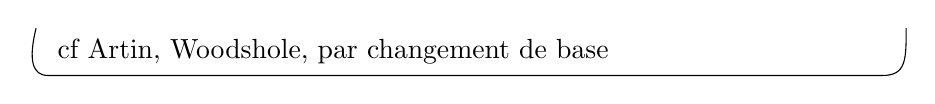
\begin{tikzpicture}\node[anchor=west] at (0,0) {cf Artin, Woodshole, par changement de base};\draw (-.15,.3) .. controls (-.25,-.1) and (-.2,-.3) .. (0,-.3)--(10.6,-.3) .. controls (10.9,-.3) and (10.9,-.1) .. (10.9,.3);\end{tikzpicture}}}

11) \uline{Supports}
\deleted{\unsure{Soient} \unsure{donc} \unsure{un} ouvert $U$ de $X$,}

\deleted{\unsure{a}} Faisceau final : $X/X$ lui-même
\[X(X')=\{e\}\]
Les sous faisceaux du faisceau final sont les ouverts de $X$.

\deleted{Support d'un $f$}
\deleted{Si $F$ est un \unsure{fai}}
La catégorie des faisceaux $F$ sur $X$ qui sur $U$ sont le faisceau final équivaut à la catégorie des faisceaux sur $Y=X-U$, par le foncteur image directe.

De $=$, faisceaux abéliens sur $X$ nuls sur $U$ $=$ faisceaux abéliens sur $Y$.

Support d'un faisceau abélien
\deleted{$\Gamma_Y(F)\subset\Gamma(F)$ \unsure{Défin.}}

Support d'une section d'un faisceau abélien
\[
\Gamma_Y(F)\subset\Gamma(F)
\]
\[
\underline\Gamma_Y(F)\subset F
\qquad
\underline\Gamma_Y(F)(X')=\Gamma_{Y'}(X',F')
\]

Foncteurs dérivés
\[
\left\{\begin{aligned}
H^i_Y(X,F)&\simeq\operatorname{Ext}^i(X;\mathbf Z_Y,F)\\
\underline H^i_Y(F)&\simeq\underline{\operatorname{Ext}}^i(\mathbf Z_Y,F)\\
&\text{'' } R^{i-1}u_*(F|U)\qquad\text{si }i\geq2
\end{aligned}\right.
\]
\margin{cf SGA 1962 ou Notes Hartshorne 1961}
\margin{si $i=0$ ou $1$, \unsure{donne} le noyau et conoyau de $F\to u_*(F)$}
\[
\text{Suite}\left\{\begin{array}{l}\text{exacte}\\\text{spectrale.....}\end{array}\right.
\]

12) \uline{Pureté}
\diagram{\begin{tikzcd}
Y \arrow[rr,phantom,"\subset"] \arrow[dr,no head,"\text{lisse}"'] && X \arrow[dl,no head,"\text{lisse}"]\\
& k &
\end{tikzcd}}
réguliers, $\operatorname{codim}_X(Y)=p$ en chaque pt de $Y$
\[
\left\{\begin{aligned}
\underline H^i_Y((\mathbf Z/n\mathbf Z)_X)&=0&&\text{si }i\neq2p\\
&\simeq\mu_n^{\otimes(-p)}&&\text{si }i=2p
\end{aligned}\right.
\]
\margin{$n$ premier aux car. résiduelles de $Y$}
\margin{Donner \unsure{définition} de la classe fondamentale \deleted{$X$ \unsure{lisse}} locale}
\mspage{11}
\scanpage{13}
- 194 - \hfill n\textsuperscript{o} 391

5. \uline{Systèmes de type} $A_\ell$, $(\ell\geq1)$.

(I) Considérons dans l'espace $V=\mathrm R^{\ell+1}$ l'intersection du réseau $L_{\unsure{o|0}}$, (n\textsuperscript{o} 4), et de l'hyperplan $V'$ d'équation $\sum_{i=1}^{\ell+1}\xi_i=0$ ; c'est un réseau $L'_{\unsure{o|0}}$ dans $V$ ; la valeur minima de $(u|u)$ dans $L'_{\unsure{o|0}}$ est $2$ et elle est atteinte pour les vecteurs de la forme $\varepsilon_i-\varepsilon_j$, $(i\neq j,\ 1\leq i\leq\ell+1,\ 1\leq j\leq\ell+1)$. Montrons que l'ensemble $R$ de ces vecteurs est un \uline{système de racines}, (évidemment réduit), dans $V'$. En effet, il est clair que pour $u$, $v$ dans $R$, $2(u|v)/(u|u)$ est entier puisque $(u|u)=2$ et la conclusion résulte du n\textsuperscript{o} 4. Le nombre des racines $n$ est $\ell(\ell+1)$.

(II) Posons :
\[
\alpha_1=\varepsilon_1-\varepsilon_2\ ,\quad
\alpha_2=\varepsilon_2-\varepsilon_3\ ,\ldots,\quad
\alpha_\ell=\varepsilon_\ell-\varepsilon_{\ell+1}\ .
\]
Il est immédiat que tout élément de $R$ est combinaison linéaire des $\alpha_i$, $(1\leq i\leq\ell)$, à coefficients tous $\geq0$ ou tous $\leq0$ ; donc, (§ 6, n\textsuperscript{o} 7, cor. 3 de la prop. 14), les $\alpha_i$ forment un système de \uline{racines simples} $S$ de $R$. En outre, on a $\|\alpha_i\|^2=2$ pour tout $i$, $(\alpha_i|\alpha_{i+1})=-1$ pour $1\leq i\leq\ell-1$ et $(\alpha_i|\alpha_j)=0$ pour $j>i+1$ ; le schéma de Dynkin de $R$ est donc du type $A_\ell$, ce qui montre que $R$ est irréductible.

(III) En vertu du § 8, n\textsuperscript{o} 3, formule (4), on a $h=n/\ell=\ell+1$.

(IV) L'ordre de la plus grande racine est $h-1=\ell$, (§ 8, n\textsuperscript{o} 5, prop. 6). Or, $\varepsilon_1-\varepsilon_{\ell+1}=\alpha_1+\alpha_2+..+\alpha_\ell$ est une racine positive d'ordre $\ell$ ; donc c'est la plus grande racine $\widetilde\alpha$, (§ 6, n\textsuperscript{o} 6, prop. 13). Elle est orthogonale à toutes les racines simples sauf à $\alpha_1$ et $\alpha_\ell$, et on a $(\widetilde\alpha|\alpha_1)=(\widetilde\alpha|\alpha_\ell)=1$.
\mspage{12}
\scanpage{14}
\figure{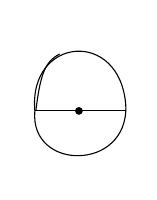
\begin{tikzpicture}[scale=.7]
\draw (0,0) .. controls (-.12,1.35) and (1.55,1.5) .. (1.65,.1) .. controls (1.7,-1.1) and (-.1,-1.1) .. (0,0);
\draw (0,0)--(1.65,0);\fill (.8,0) circle (2pt);
\draw (.02,.02) .. controls (.1,.65) and (.18,.9) .. (.45,1.03);
\end{tikzpicture}}
NB
\[
\mu_n=\operatorname{Ker}(G_m\xrightarrow{n}G_m)
\]
\[
\mu_n(X')=\deleted{\operatorname{Ker}}{}_n\Gamma(X',\mathcal O_{X'})^*
\]
\margin{$\mu_n$ fini plat sur $X$}

Si $n$ premier aux car de $X$, $\mu_{nX}$ est \uline{étale} sur $X$ loc. isom. (pour top. étale) à $\mathbf Z/n\mathbf Z$. Il n'faut surtout pas les confondre. Les $\mu_{nX}^{\otimes d}$ $(d\in\mathbf Z)$ sont donc définis, et sont \inserted{loc} isomorphes à $(\mathbf Z/n\mathbf Z)_X$ [le choix d'une section primitive de $\mu_n$ définit un isom $\mu_{nX}^{\otimes d}\simeq(\mathbf Z/n\mathbf Z)_X$, multiplier cette section par $\lambda\in\mathbf Z/n\mathbf Z$ multiplie l'isom précédent par $\lambda^d$ ...]. \uline{Dém} presque immédiate par th. de changement de base......

\uline{Pb} \fbox{Pureté ``absolue''} \unsure{avec|sans} hypothèse de \unsure{lissité} remplacée par hyp. de régularité. OK. \inserted{pour bons premiers} en égales car. quand on dispose de la résolution des singularités (Artin).

Il y a aussi un th de pureté relatif sur une base quelconque ....

\deleted{13)}

Extension aux div. à croisements normaux....

\deleted{13) \uline{Les} $R^i_!f_*(F)$.

Morphismes \unsure{compactifiables} $f:X\to Y$.
\unsure{On factorise en} $\unsure{X'}\xrightarrow{i}\overline X\ \unsure{\perp}\ Y$, où $i$ : \unsure{imm.}}
\mspage{13}
\scanpage{15}
- 193 - \hfill n\textsuperscript{o} 391

(I) Les racines et leur nombre.

(II) Un système de racines simples $S$.

(III) Le nombre de Coxeter.

(IV) La plus grande racine, (relative à $S$), et les racines de $S$ qui ne lui sont pas orthogonales ; en joignant ces dernières, (dans le schéma de Dynkin), par un trait pointillé à un point hors du schéma représentant la plus grande racine, (affecté s'il y a lieu de la longueur de cette dernière), on obtiendra ce qu'on appelle le \uline{schéma de Dynkin complété}.

(V) Les coracines et la forme bilinéaire canonique, (proportionnelle à la forme métrique $(x|y)$ de $V$).

(VI) Les poids fondamentaux, (relatifs à $S$).

(VII) La somme des racines positives, (pour $S$).

(VIII) Le groupe $\Gamma(R)/\Gamma_{\unsure{o|0}}(R)$ et l'indice de connexion.

(IX) Les exposants, (et éventuellement les invariants symétriques).

(X) L'ordre du groupe de Weyl, (et éventuellement sa structure).

(XI) Les automorphismes du schéma de Dynkin.

Pour chacun des 9 types de schémas de Dynkin, ces données seront rassemblées dans les planches II à X, en les ordonnant de façon uniforme comme ci-dessus.
\mspage{14}
\scanpage{16}
\deleted{ouverte, et $\overline f$ propre. Ex! \unsure{un morphisme} quasi-projectif sur $Y$ \unsure{ou prop.}}

13) \uline{Faisceaux} \uline{constructibles}

Faisceaux loc. \deleted{\unsure{isom.}} constants

Faisceau constructibles : en général, il est loc. constant à fibres \deleted{finies} de t.f. sur des ens loc fermés cons. qui partitionnent $U$. Dans le cas noethérien, critère par adhérences \unsure{directes} et \deleted{\unsure{génériques}}.

\uline{Th.} Si $f:X\to Y$ \uline{propre}, $Y$ \uline{loc noeth}, alors pour tt faisceau \uline{de torsion} \uline{constructible} $F$ sur $X$, les $R^if_*(F)$ sur $Y$ sont constr.

\uline{Cor.} $X$ propre sur un corps sép. clos $k$. Alors pour tt $F$ de torsion constructible sur $X$, les $H^i(X,F)$ sont des groupes finis.

\uline{Remarques} \unsure{Question} de la généralisation
\mspage{15}
\scanpage{17}
- 192 - \hfill n\textsuperscript{o} 391

2) Le réseau $L_1$ est le sous-$\mathrm Z$-module de $L_{\unsure{o|0}}$ formé des $x=\sum_{i=1}^n\xi_i\varepsilon_i$ tels que $\sum_{i=1}^n\xi_i$ soit \uline{pair} ; comme $\xi_i$ et $\xi_i^2$ ont même parité, il revient au même de dire que $(x|x)$ est \uline{pair}. Il est engendré par les $\varepsilon_i\pm\varepsilon_j$, $(i\neq j)$.

3) Le réseau $L_2=L_{\unsure{o|0}}+\mathrm Z.(\frac12\sum_{i=1}^n\varepsilon_i)$ ; il revient au même de dire que les vecteurs $x=\sum_{i=1}^n\xi_i\varepsilon_i$ de $L_2$ sont ceux qui vérifient les relations :
\[
(4)\qquad 2\xi_i\in\mathrm Z\ ,\quad\xi_i-\xi_j\in\mathrm Z\quad\text{quels que soient }i,\ j.
\]
Comme $(\varepsilon_k|\frac12\sum_i\varepsilon_i)=\frac12$ pour tout $k$, et $\|\frac12\sum_i\varepsilon_i\|^2=n/4$, on a $(u|v)\in\frac12\mathrm Z$ pour $u$, $v$ dans $L_2$ si $n$ est pair.

4) Si $n$ est \uline{multiple de} $4$, le réseau $L_3=L_1+\mathrm Z.(\frac12\sum_{i=1}^n\unsure{\xi_i|\varepsilon_i})$, sous-$\mathrm Z$-module de $L_2$; c'est l'ensemble des vecteurs $x=\sum_{i=1}^n\xi_i\varepsilon_i$ de $V$ vérifiant les relations (4) et en outre tels que $\sum_{i=1}^n\xi_i\in2\mathrm Z$ ; on a $(u|v)\in\mathrm Z$ quels que soient $u$, $v$ dans $L_3$.

On notera que le réseau \uline{associé} à $L_{\unsure{o|0}}(V)$ est $L_{\unsure{o|0}}(V^*)$, le réseau \uline{associé} à $L_1(V)$, (resp. $L_2(V)$), est $L_2(V^*)$, (resp. $L_1(V^*)$) ; enfin, le réseau \uline{associé} à $L_3(V)$ est $L_3(V^*)$, car c'est le sous-réseau de $L_2(V^*)$ formé des $x=\sum_{i=1}^n\xi_i\varepsilon_i^*$ tels que $\frac12(\sum_{i=1}^n\xi_i)\in\mathrm Z$, et on vient de voir, (en vertu de l'hypothèse $n\equiv0\ (\operatorname{mod.}4)$) que ces conditions caractérisaient $L_3(V^*)$.

Nous allons voir successivement, dans chacun des 8 n\textsuperscript{os} suivants, comment cette méthode démontre en premier lieu l'existence des systèmes de racines correspondant aux 8 types de schémas de Dynkin autres que $G_2$ ; en outre, pour chaque type de schéma, nous expliciterons :
\mspage{16}
\scanpage{18}
à des $f$ de type fini au lieu de $f$ propre. Se ramène au cas d'une \uline{imm.} \uline{ouverte}. Se résoud par l'affirmative lorsqu'on dispose de la résolution des singularités \inserted{$+$ pureté}, p.ex. en car. $0$ \inserted{pour ``bons \unsure{préschémas|premiers}''}, \unsure{ou plus} \inserted{bons \unsure{présch.}} \unsure{égale car.} lorsqu'on dispose de résolution des singularités \deleted{\unsure{en}} dans ce cadre....

14) \uline{Les} $R^i_!f_*(F)$.

Soit $f:X\to Y$ morphisme compactifiable, i.e. qui se factorise en
\diagram{\begin{tikzcd}
X \arrow[r,no head,"i","\text{imm. ouv.}"']&\overline X\arrow[r,"\overline f","\text{propre}"']&Y
\end{tikzcd}}
(p.ex. $f$ qu. proj. et $Y$ quasi-cpt).

Pour tt faisceau de torsion $F$ sur $X$, considérons $i_!(F)$ [exact en $F$] puis les $R^q_{\unsure{\deleted{!}|\xi}}\overline f_*(i_!(F))$, forment un foncteur coh. en $F$. Il résulte de façon quasi-triviale du th. de changement de base que ce foncteur coh.
\mspage{17}
\scanpage{19}
- 191 - \hfill n\textsuperscript{o} 391

racines de $R$ sont telles que $(u|u)=1$ ou $(u|u)=2$, (en excluant le cas des systèmes de racines de type $G_2$, dont la structure a été déterminée au § 6, n\textsuperscript{o} 12). Inversement, partons d'un réseau $L$ dans un espace euclidien $V$, et soit $R$ la partie formée de \uline{tous} les vecteurs de $L$ tels que $(u|u)=\lambda$, (ou vérifiant l'une des deux conditions $(u|u)=\lambda$, $(u|u)=2\lambda$), pour un $\lambda$ convenable. Alors, si $R$ engendre $V$ et si on suppose de plus que pour tout couple $(u,v)$ de vecteurs de $R$, le nombre $2(u|v)/(u|u)$ est \uline{entier}, $R$ est un \uline{système de racines} : en effet, si $s_u$ est la réflexion orthogonale de vecteur $u$, $s_u(v)$ appartient alors au sous-groupe de $V$ engendré par $u$ et $v$, donc \uline{a fortiori} à $L$, et en outre $s_u(v)$ a même norme que $v$, donc est dans $R$, ce qui prouve $(\mathrm{SR}_{\mathrm I})$ ; comme $(\mathrm{SR}_{\mathrm{II}})$ et $(\mathrm{SR}_{\mathrm{III}})$ sont vérifiés par hypothèse, cela prouve notre assertion. Il restera naturellement à vérifier dans chaque cas que le système $R$ est réduit et irréductible.

Nous allons voir qu'il est possible d'obtenir tous les systèmes de racines correspondant aux schémas de Dynkin du th. 2, ($G_2$ exclus), en prenant pour $V$ un espace numérique $\mathrm R^n$, dont nous désignerons par $\varepsilon_i$, $(1\leq i\leq n)$, la base canonique, ($(\varepsilon_i^*)$ étant la base duale), et où la forme métrique admet $(\varepsilon_i)$ pour \uline{base orthonormale} ; on considérera alors dans $V$ les réseaux $L_i$, $(i=0,1,2,3)$, suivants notés aussi $L_i(V)$, (et leurs intersections par certains sous-espaces de $V$) :

1) Le réseau $L_{\unsure{o|0}}$ est le $\mathrm Z$-module de base $(\varepsilon_i)$ ; il est clair que $(u|v)$ est entier pour $u$, $v$ dans $L_{\unsure{o|0}}$. En outre, les vecteurs de $L_{\unsure{o|0}}$ tels que $(u|u)=1$ sont les vecteurs $\pm\varepsilon_i$, $(1\leq i\leq n)$ ; ceux pour lesquels $(u|u)=2$ sont les vecteurs $\pm\varepsilon_i\pm\varepsilon_j$ pour $i\neq j$.
\mspage{18}
\scanpage{20}
à isom près est \uline{indépendant} du choix de la factor. Notation $R^q_!f_*(F)$.
\[
R^0_!f_*(F)=(f_!(F))=\text{image directe à supp. propre sur }Y.
\]
\deleted{Propriétés} Propriétés plus importantes : \unsure{certaines} \unsure{égales} que $R^qf_*(F)$, en \uline{aussi bon que si $f$ propre}

(i) \uline{Comparaison avec cas classique} sur $\mathbf C$

(ii) \uline{Th. de changement de base} \deleted{\unsure{cf}}, \uline{dim} \uline{coh.}

(iii) \deleted{\uline{Suite spectrale de Leray}} \inserted{Th. de finitude}

(iv) Suite spectrale de Leray

\margin{phénomènes spéciaux}
(v) Si $f$ quasi-fini \inserted{\unsure{sép.}} alors les $R^i_!f_*(F)=0$

\deleted{\unsure{D'autre part}}
(vi) Si $f$ \uline{étale}, on a un hom can.
\[
\operatorname{Tr}_f(F):f_!(F)\mathbin{-}F
\]
[d'où la covariance, pour $f:X'\mathbin{-}X$ morphismes étales -- p.ex. immersions ouvertes -- ] des préschémas compactifiables sur $Y$
\[
R^q_!g'_*(F')\mathbin{-}R^q_!g_*(f_!(F'))
\]
ou encore
\[
R^q_!g'_*(f^*(F))\longrightarrow R^q_!g_*(F)
\]
]

(vi) \uline{suite exacte de cohomologie relative}
\mspage{19}
\scanpage{21}
- 189 - \hfill n\textsuperscript{o} 391

En effet, (§ 6, n\textsuperscript{o} 5, prop. 12), ce groupe quotient est isomorphe au sous-groupe $G_{\unsure{o|0}}$ de $A(R)$ laissant stable un système de racines simples $S(C)$ de $R$ ; il est clair que tout élément de $G_{\unsure{o|0}}$ détermine un automorphisme unique du schéma de Dynkin de $R$ relatif à $C$ ; mais inversement, un tel automorphisme se prolonge en un automorphisme unique de $R$ en vertu de la prop. 2, d'où le corollaire.

Les remarques du début et les définitions précédentes montrent que le schéma de Dynkin d'un système de racines $R$, relatif à un système de racines simples $(v_i)_{1\leq\unsure{j|i}\leq\ell}$, détermine le schéma de Coxeter du groupe de Weyl $W(R)$ de la manière suivante : les graphes sous-jacents sont les mêmes ; en outre, si $\{v_i,v_j\}$ est une arête du schéma de Dynkin, le nombre $m_{ij}$ est égal à $3$ si $f(v_i)=f(v_j)$, à $4$ si $f(v_i)/f(v_j)$ est égal à $\frac12$ ou à $2$, à $6$ si $f(v_i)/f(v_j)$ est égal à $1/3$ ou à $3$. On verra par contre ci-dessous qu'un même schéma de Coxeter peut correspondre à deux schémas de Dynkin non isomorphes, (en fait, il ne peut correspondre qu'à \uline{deux} tels schémas au plus, et cela ne se produit que pour les schémas de Coxeter de type $B_\ell$ ; pour tous les autres types, le schéma de Coxeter de $W(R)$ détermine le schéma de Dynkin de $R$ à isomorphisme près).

THEOREME 2.- \uline{Si} $R$ \uline{est un système de racines réduit irréductible}, \uline{son schéma de Dynkin est nécessairement isomorphe à l'un des suivants}, (\uline{qui sont deux à deux non isomorphes}) :

\figure{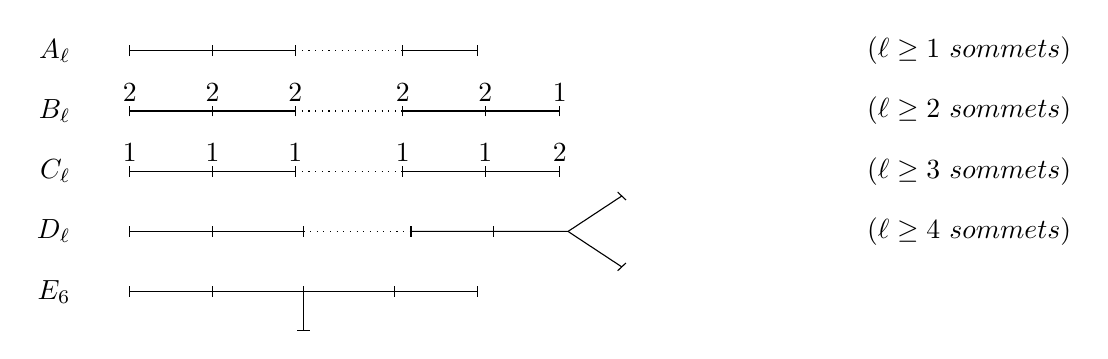
\begin{tikzpicture}[x=1.05cm,y=.9cm]
\node[left] at (-.6,0) {$A_\ell$};
\draw (0,0)--(2,0);\draw[dotted] (2,0)--(3.3,0);\draw (3.3,0)--(4.2,0);
\foreach \x in {0,1,2,3.3,4.2}{\draw (\x,-.075)--(\x,.075);}
\node[right] at (8.8,0) {$(\ell\geq1\ \uline{\text{sommets}})$};
\node[left] at (-.6,-.85) {$B_\ell$};
\draw (0,-.85)--(2,-.85);\draw[dotted] (2,-.85)--(3.3,-.85);\draw (3.3,-.85)--(5.2,-.85);
\foreach \x in {0,1,2,3.3,4.3,5.2}{\draw (\x,-.925)--(\x,-.775);}
\foreach \x in {0,1,2,3.3,4.3}{\node[above] at (\x,-.85) {$2$};}\node[above] at (5.2,-.85) {$1$};
\node[right] at (8.8,-.85) {$(\ell\geq2\ \uline{\text{sommets}})$};
\node[left] at (-.6,-1.7) {$C_\ell$};
\draw (0,-1.7)--(2,-1.7);\draw[dotted] (2,-1.7)--(3.3,-1.7);\draw (3.3,-1.7)--(5.2,-1.7);
\foreach \x in {0,1,2,3.3,4.3,5.2}{\draw (\x,-1.775)--(\x,-1.625);}
\foreach \x in {0,1,2,3.3,4.3}{\node[above] at (\x,-1.7) {$1$};}\node[above] at (5.2,-1.7) {$2$};
\node[right] at (8.8,-1.7) {$(\ell\geq3\ \uline{\text{sommets}})$};
\node[left] at (-.6,-2.55) {$D_\ell$};
\draw (0,-2.55)--(2.1,-2.55);\draw[dotted] (2.1,-2.55)--(3.4,-2.55);\draw (3.4,-2.55)--(5.3,-2.55)--(5.95,-2.05);\draw (5.3,-2.55)--(5.95,-3.05);
\foreach \x in {0,1,2.1,3.4,4.4}{\draw (\x,-2.625)--(\x,-2.475);}
\draw (5.9,-1.995)--(6,-2.105);\draw (5.9,-3.105)--(6,-2.995);
\node[right] at (8.8,-2.55) {$(\ell\geq4\ \uline{\text{sommets}})$};
\node[left] at (-.6,-3.4) {$E_6$};
\draw (0,-3.4)--(4.2,-3.4);\foreach \x in {0,1,2.1,3.2,4.2}{\draw (\x,-3.475)--(\x,-3.325);}
\draw (2.1,-3.4)--(2.1,-3.95);\draw (2.025,-3.95)--(2.175,-3.95);
\end{tikzpicture}}
\mspage{20}
\scanpage{22}
\textcircled{\mspage{15}}

On fixe entier $n$ premier aux car. résiduelles

\uline{Classe fondamentale locale}

Supposons $Y\longrightarrow X$ ``intersection complète de dim relative $1$'' et supposons d'abord $Y=V(\varphi)$, $\varphi$ section régulière de $\mathcal O_X$. Alors si $u:X-Y=U\to X$, donc \deleted{$\unsure{i|u}_*(\mathcal O_U)\sim\mathcal O_X[\frac1\varphi]$},
\deleted{$\unsure{i|u}_*(\mathcal O_U^*)$ \unsure{$\to$}}
\[
\varphi\in\Gamma(\unsure{i|u}_*(G_{mU}))
\]
\deleted{$\text{et }\unsure{n}\in\Gamma(X,\unsure{i|u}_*(G_{mU}^*))$}

\deleted{D'où} alors $\varphi$ est déterminé \inserted{par $Y$} mod multiplication par un $\in\Gamma(X,\unsure{i|u}_*(G_{mX}))$, donc \deleted{l'image} $\varphi$ définit une section \deleted{$\varphi\in$} \uline{canonique} de \deleted{$\unsure{i|u}_*(\mathcal O_U^*)/$} $\unsure{i|u}_*(G_{mU})/G_{mX}$. Or on a la suite exacte canonique
\diagram{\begin{tikzcd}[column sep=small]
0\arrow[r]&\underline H^0_Y(G_{mX})\arrow[r]\arrow[d,equal]&G_{mX}\arrow[r,no head]&i_*(G_{mU})\arrow[r,no head,"d"]&\underline H^1_Y(G_{mX})\arrow[d]\\
&0&&&0
\end{tikzcd}}
qui donne ici
\[
\deleted{\unsure{H^1}}\ \underline H^1_Y(G_{mX})\xrightarrow{\sim}i_*(G_{mU})/\operatorname{Im}G_{mX}\ ,
\]
et montre que $d\varphi$ est une section \uline{canonique} de $\underline H^1_Y(G_{mX})$, que nous allons noter \deleted{$\unsure{\varepsilon}_{Y/X}$} $\underline{\unsure{\beta}}_{Y/X}$. D'autre part, on a \uline{la} suite exacte de Kummer
\[
0\mathbin{-}\mu_{nX}\longrightarrow G_{mX}\mathrel{\overset{n}{-}}G_{mX}\longrightarrow0
\]
\mspage{21}
\scanpage{23}
- 218 - \hfill n\textsuperscript{o} 391

(VII) La demi-somme des racines positives est la somme des poids fondamentaux, (§ 6, n\textsuperscript{o} 9, prop. 8), et vaut donc :
\[
\begin{aligned}
\rho&=\varepsilon_2+2\varepsilon_3+3\varepsilon_4+4\varepsilon_5+4(\varepsilon_8-\varepsilon_7-\varepsilon_6)=\\
&=8\alpha_1+11\alpha_2+15\alpha_3+21\alpha_4+15\alpha_5+8\alpha_6.
\end{aligned}
\]

(VIII) De même qu'au n\textsuperscript{o} 11, le réseau des vocables $\Gamma_{\unsure{o|0}}(R'')$ est l'associé \uline{dans} $V''$ du réseau $\Gamma_2^*$ de $V''{}^*$ \uline{projection orthogonale} dans $V''{}^*$ de $\Gamma_{\unsure{o|0}}(R^*)$, (lorsque $V''{}^*$ est identifié au sous-espace de $V^*$ orthogonal à $\varepsilon_7^*+\varepsilon_8^*$ et $\varepsilon_7^*-\varepsilon_6^*$). Le groupe $\Gamma(R'')/\Gamma_{\unsure{o|0}}(R'')$ est donc \uline{isomorphe au groupe} $\Gamma_2^*/\Gamma_{\unsure{o|0}}(R''{}^*)$, qu'il reste à calculer. Or, les projections orthogonales de $\varepsilon_8^*$, $-\varepsilon_7^*$ et $-\varepsilon_6^*$ sur $V''{}^*$ sont toutes trois égales $\frac13(\varepsilon_8^*-\varepsilon_7^*-\varepsilon_6^*)$ et les autres $\varepsilon_i^*$ sont dans $V''{}^*$ ; on en déduit aisément que $\Gamma_2^*$ est engendré par $\Gamma_{\unsure{o|0}}(R''{}^*)$ et par l'unique vecteur $\mu^*=\frac13(\varepsilon_8^*-\varepsilon_7^*-\varepsilon_6^*)$ ; mais comme $3\mu^*\in\Gamma_{\unsure{o|0}}(R''{}^*)$, on voit que $\Gamma_2^*/\Gamma_{\unsure{o|0}}(R''{}^*)$ est isomorphe à $\mathrm Z/3\mathrm Z$ et par suite $\Gamma(R'')/\Gamma_{\unsure{o|0}}(R'')$ est \uline{isomorphe à} $\mathrm Z/3\mathrm Z$, et l'indice de connexion $f=3$.

(IX) et (X). Le calcul de la plus grande racine et de l'indice de connexion permet, grâce au § 6, n\textsuperscript{o} 10, prop. 23, de calculer l'ordre du groupe de Weyl $W(R'')$, qui est égal à :
\[
6!1.2.2.3.2.1.3=2^7.3^4.5=51.840.
\]
La suite des exposants a 6 termes compris entre 1 et 11, et comprend les termes 1, 5, 7, 11 qui sont étrangers à 12, (§ 8, n\textsuperscript{o} 5, prop. 6). Les deux derniers termes de la suite $m$, $m'$ sont des entiers tels que :
\[
m+m'=12
\]
\[
(m+1)(m'+1)(1+1)(5+1)(7+1)(12+1)=2^7.3^4.5
\]
\mspage{22}
\scanpage{24}
d'où
\[
\unsure{\partial_n|\delta_n}:\underline H^1_Y(G_{mX})\longrightarrow\underline H^2_Y(\mu_{nX})
\]
et nous posons
\[
\deleted{\unsure{\varphi}}\ \underline{\unsure{\gamma|\sigma}}_{Y/X}^{(n)}=\unsure{\partial_n|\delta_n}(\underline\beta_{Y/X})\in\Gamma(X,\underline H^2_Y(\mu_{nX}))
\]
en laissant tomber les exposants $n$ s'il n'y a pas d'ambiguïté possible.

\inserted{La définition de} Cette section \deleted{satisfait} commute à la localité de Zariski (et $=$ à tt changement de base $X'\to X$ tel que $Y'$ reste une ``int. complète'' i.e. $\varphi'$ reste section régulière) ce qui permet de définir $\gamma_{Y/X}^{(n)}$ en général (sans équation globale). Si \inserted{maintenant} $Y$ est intersection complète de codim $d$, alors \unsure{localt} $Y$ est de la forme
\[
Y=Y_1\cap\ldots\cap Y_d
\]
et on posera
\[
\underline{\unsure{\gamma|\sigma}}_{Y/X}
=\underline{\unsure{\gamma|\sigma}}_{Y_1/X}^{\deleted{\unsure{(n)}}}\ .\ \ldots\ .\ \underline{\unsure{\gamma|\sigma}}_{Y_d/X}
\in\Gamma(Y,\underline H^{2d}_Y(\mu_n^{\otimes d}))
\]
(\uline{cup-produit}), et on prouve que cette section ne dépend pas du choix des $Y_i$, donc se définit globalement.

Propriétés générales
\mspage{23}
\scanpage{25}
- 217 - \hfill n\textsuperscript{o} 391

(IV) La racine $\frac12(\varepsilon_1+\varepsilon_2+\varepsilon_3+\varepsilon_4+\varepsilon_5-\varepsilon_6-\varepsilon_7+\varepsilon_8)$ est la plus grande des racines de $R''$ pour l'ordre induit par celui considéré sur $\mathrm R^8$, (n\textsuperscript{o} 10) ; c'est donc la plus grande racine $\widetilde\alpha$, (§ 6, n\textsuperscript{o} 6, cor. 2 de la prop. 13) ; on a $\widetilde\alpha=\alpha_1+2\alpha_2+2\alpha_3+3\alpha_4+2\alpha_5+\alpha_6$, et on vérifie que son ordre est $h-1=11$. Cette racine est orthogonale à toutes les racines simples $\alpha_i$, $(1\leq i\leq6)$, sauf $\alpha_2$, et l'on a $(\widetilde\alpha|\alpha_2)=1$.

(V) Le même raisonnement qu'au n\textsuperscript{o} 11 montre que les \uline{coracines} de $R''$ s'obtiennent en remplaçant $\varepsilon_i$ par $\varepsilon_i^*$ dans les expressions des racines de $R''$, et $R''{}^*$ est isomorphe à $R''$. Toutes les racines ayant la même longueur, la \uline{forme bilinéaire canonique} pour $R$ est $(x|y)/2h=(x|y)/24$ et la longueur des racines est $1/2\sqrt3$, (§ 8, n\textsuperscript{o} 5, \uline{Remarque}). Le nombre des racines non orthogonales à une racine donnée est $4h-6=42$ et le nombre $\gamma$ est égal à $h^2=144$.

(VI) Le calcul des poids fondamentaux, formant la base duale de $(\alpha_i^*)$, $(1\leq i\leq6)$, dans $V''$, donne :
\[
\omega_1=\frac23(\varepsilon_8-\varepsilon_7-\varepsilon_6)=\frac13(4\alpha_1+3\alpha_2+5\alpha_3+6\alpha_4+4\alpha_5+2\alpha_6)
\]
\[
\begin{aligned}
\omega_2&=\frac12(\varepsilon_1+\varepsilon_2+\varepsilon_3+\varepsilon_4+\varepsilon_5-\varepsilon_6-\varepsilon_7+\varepsilon_8)=\\
&=\alpha_1+2\alpha_2+2\alpha_3+3\alpha_4+2\alpha_5+\alpha_6=\widetilde\alpha
\end{aligned}
\]
\[
\begin{aligned}
\omega_3&=\frac56(\varepsilon_8-\varepsilon_7-\varepsilon_6)+\frac12(-\varepsilon_1+\varepsilon_2+\varepsilon_3+\varepsilon_4+\varepsilon_5)=\\
&=\frac13(5\alpha_1+6\alpha_2+10\alpha_3+12\alpha_4+8\alpha_5+4\alpha_6)
\end{aligned}
\]
\[
\omega_4=\varepsilon_3+\varepsilon_4+\varepsilon_5-\varepsilon_6-\varepsilon_7+\varepsilon_8=2\alpha_1+3\alpha_2+4\alpha_3+6\alpha_4+4\alpha_5+2\alpha_6
\]
\[
\begin{aligned}
\omega_5&=\frac23(\varepsilon_8-\varepsilon_7-\varepsilon_6)+\varepsilon_4+\varepsilon_5=\\
&=\frac13(4\alpha_1+6\alpha_2+8\alpha_3+12\alpha_4+10\alpha_5+5\alpha_6)
\end{aligned}
\]
\[
\begin{aligned}
\omega_6&=\frac13(\varepsilon_8-\varepsilon_7-\varepsilon_6)+\varepsilon_5=\\
&=\frac13(2\alpha_1+3\alpha_2+4\alpha_3+6\alpha_4+5\alpha_5+4\alpha_6).
\end{aligned}
\]
\mspage{24}
\scanpage{26}
\margin{\uline{propriétés} \uline{caractéristiques}}
\[
\left\{\begin{array}{ll}
\text{(i)} & \text{Compatibilité aux chgts de base admissibles}\\[4pt]
\text{(ii)} & \text{Si }Y=V(\varphi),\quad \underline\gamma_{Y/X}^{(n)}=d(\beta_{Y/X}^{(n)})\text{ comme dessus.}\\[4pt]
\text{(iii)} & \underline\gamma_{Y.Y'/X}^{(n)}=\underline\gamma_{Y/X}^{(n)}\cdot\underline\gamma_{Y'/X}^{(n)}
\end{array}\right.
\]
si $Y.Y'$ ``sans dim. excédentaire''

\[\Downarrow\]
(iv) Compatibilité pour $n$ variable

( \uline{NB} La ``bonne'' classe se trouve dans
$\Gamma(Y,\underline H^{2d}_Y(\mathbf Z_\ell(d)))$, il y en a une pour tt $\ell$ premier aux car. résiduelles de $Y$ ).

\uline{Application à la construction de classes de coh. associées à certains cycles.}

Supposons $\underline H^i_Y((\mathbf Z/n\mathbf Z)_X)=0$ \deleted{\unsure{qt}} quand $i<2d$

d'où également
\[
\underline H^i_Y(\mu_{nX}^{\otimes d})=0\qquad\text{pour }i<2d
\]
C'est la situation du th. de pureté, vrai

(i) $X,Y$ lisses sur une base $S$

(ii) $Y,X$ réguliers, $X$ excellent, car. nulles

(iii) $d=1$, $X$ normal.
\mspage{25}
\scanpage{27}
\begin{center}- 216 -\end{center}
\hfill n° 391

(§ 8, n° 3, formule (2)) ; autrement dit, la suite des exposants est :
\[
1,\ 5,\ 7,\ 9,\ 11,\ 13,\ 17.
\]
(X) On déduit de (IX) et du § 8, n° 3, cor. 1 de la prop. 3, que l'ordre du groupe de Weyl $W(R)$ est :
\[
2.6.8.10.12.14.18=2^{10}.3^4.5.7.
\]
(XI) Le même raisonnement qu'au n° 8 montre que le seul automorphisme du schéma de Dynkin $E_7$ est l'identité.

12. \uline{Système de type} $E_6$.

(I) Gardons toujours les notations du n° 10, et considérons l'intersection $R''$ de $R$ et du sous-espace $V''$ de codimension 2, orthogonal aux deux vecteurs $\varepsilon_8+\varepsilon_7$ et $\varepsilon_7-\varepsilon_6$ ; ce sont donc les vecteurs $x=\sum_{i=1}^8\xi_i\varepsilon_i$ de $R$ tels que $\xi_8=-\xi_7=-\xi_6$, autrement dit :
\[
\pm\varepsilon_i\pm\varepsilon_j,\ (i\ne j,\ 1\leq i\leq5,\ 1\leq j\leq5)
\]
\[
\pm\frac12(\varepsilon_8-\varepsilon_7-\varepsilon_6+\sum_{i=1}^5(-1)^{\unsure{\nu(i)}}\varepsilon_i)\quad\text{où la somme }\sum_{i=1}^5\unsure{\nu(i)}\text{ est}
\]
\uline{paire}.

Il est clair que $R''$ engendre $V''$, donc est un système de racines réduit de rang 6, ayant $n=\binom52.4+2^5=72$ éléments.

(II) Si l'on exprime qu'une racine $\sum_{i=1}^8n_i\alpha_i$ de $R$ est orthogonale à la fois à $\varepsilon_8+\varepsilon_7$ et à $\varepsilon_7-\varepsilon_6$, il vient, en vertu du n° 10, (II), $n_8=n_7=0$. Le même raisonnement que dans le n° 11 montre alors que les $\alpha_i$ pour $1\leq i\leq6$ forment un système de \uline{racines simples} $S''$ de $R''$. Le calcul des $(\alpha_i|\alpha_j)$ fait au n° 10 montre que le schéma de Dynkin de $R''$ est de type $E_6$, et $R''$ est irréductible.

(III) En vertu du § 8, n° 3, formule (4), on a $h=n/\ell=12$.
\mspage{26}
\scanpage{28}
Alors la suite spectrale implique
\[
H^i_Y(X,\mu_{nX}^{\otimes d})=0\qquad\text{si }i<2d
\]
\[
H^{2d}_Y(X,\mu_{nX}^{\otimes d})\simeq\Gamma(Y,\underline H^{2d}_Y(\deleted{\unsure{\mathbf Z/n\mathbf Z}}\mu_{nX}^{\otimes d}))
\]
d'où un \deleted{\unsure{hom} canonique} élément canonique
\[
\gamma_{X/Y}^{(n)}\in H^{2d}_Y(X,\mu_{nX}^{\otimes d})
\]
[qu'on peut maintenant spécialiser dans $H^{2d}_{\deleted{\unsure{Y}}}(X,\mu_{nX}^{\otimes d})$, ou si $X$ est propre sur un $S$ dans
\[
H^{2d}_{\Phi_{Y/X}}(X,\mu_{nX}^{\otimes d}).
\]
\margin{$\Phi_{Y/X}\ \longrightarrow\ \text{famille de \unsure{cpts}}$}

\margin{N.B ($\beta_{Y/X}\in H^1_Y(X,G_{mX})$ et $\gamma^{(n)}_{Y/X}=\partial_n(\beta_{Y/X})$, en particulier son image dans $H^2_Y(X,G_{mX})$ est nulle)}

\uline{Exemple 1}. $X$ lisse sur $k$ \inserted{sép. clos.}, \deleted{$x$ pt} dim relative $d$, \deleted{\unsure{il va résulter des} $\unsure{C}$ \unsure{th. de}} \inserted{$x$ pt de $X$ \unsure{rat} sur $k$, d'où}
\[
\gamma_{x/X}\in H^{2d}_!(X,\mu_{nX}^{\otimes d}).
\]
Il va résulter de le théor. qu'on va \unsure{prouver} que \deleted{\unsure{pour} $\unsure{A}$} si $X$ est géom. connexe, cet élément est \uline{une base} \uline{de} $H^{2d}_!(X,\mu_{nX}^{\otimes d})$ \uline{et ne dépend pas du choix de $x$}; \deleted{\unsure{ici}} C'est qu'on avait vérifié directement dans le cas où $d=1$, en \deleted{\unsure{le compa}} \inserted{nous \unsure{ramenant}} au cas où $C$ étant complet et où on dispose déjà
\mspage{27}
\scanpage{29}
\begin{center}- 214 -\end{center}
\hfill n° 391

son ordre est $h-1=17$. Elle est orthogonale à toutes les racines simples sauf à $\alpha_1$ et l'on a $(\widetilde\alpha|\alpha_1)=1$.

(V) Ce qui a été vu au n° 10 montre que les \uline{coracines} de $R'$ s'obtiennent encore en remplaçant $\varepsilon_i$ par $\varepsilon_i^*$ dans les expressions des racines de $R'$, et $R'^*$ est donc isomorphe à $R'$. Toutes les racines ayant même longueur, la \uline{forme bilinéaire canonique} pour $R$ est $(x|y)/2h=(x|y)/36$ et la longueur des racines est $1/3\sqrt2$, (§ 8, n° 5, \uline{Remarque}). Le nombre des racines non orthogonales à une racine donnée est $4h-6=66$ et le nombre $\gamma$ est égal à $h^2=2^2.3^4$.

(VI) Le calcul des poids fondamentaux, formant la base duale de $(\alpha_i^*)$, $(1\leq i\leq7)$, dans $V'$, donne :
\[
\omega_1=\varepsilon_8-\varepsilon_7=2\alpha_1+2\alpha_2+3\alpha_3+4\alpha_4+3\alpha_5+2\alpha_6+\alpha_7=\widetilde\alpha
\]
\[
\begin{split}
\omega_2&=\frac12(\varepsilon_1+\varepsilon_2+\varepsilon_3+\varepsilon_4+\varepsilon_5+\varepsilon_6-2\varepsilon_7+2\varepsilon_8)=\\
&=\frac12(4\alpha_1+7\alpha_2+8\alpha_3+12\alpha_4+9\alpha_5+6\alpha_6+3\alpha_7)
\end{split}
\]
\[
\begin{split}
\omega_3&=\frac12(-\varepsilon_1+\varepsilon_2+\varepsilon_3+\varepsilon_4+\varepsilon_5+\varepsilon_6-3\varepsilon_7+3\varepsilon_8)=\\
&=3\alpha_1+4\alpha_2+6\alpha_3+8\alpha_4+6\alpha_5+4\alpha_6+2\alpha_7
\end{split}
\]
\[
\begin{split}
\omega_4&=\varepsilon_3+\varepsilon_4+\varepsilon_5+\varepsilon_6+2(\varepsilon_8-\varepsilon_7)=\\
&=4\alpha_1+6\alpha_2+8\alpha_3+12\alpha_4+9\alpha_5+6\alpha_6+3\alpha_7
\end{split}
\]
\[
\begin{split}
\omega_5&=\frac12(2\varepsilon_4+2\varepsilon_5+2\varepsilon_6+3(\varepsilon_8-\varepsilon_7))=\\
&=\frac12(6\alpha_1+9\alpha_2+12\alpha_3+18\alpha_4+15\alpha_5+10\alpha_6+5\alpha_7)
\end{split}
\]
\[
\omega_6=\varepsilon_5+\varepsilon_6-\varepsilon_7+\varepsilon_8=2\alpha_1+3\alpha_2+4\alpha_3+6\alpha_4+5\alpha_5+4\alpha_6+2\alpha_7
\]
\[
\omega_7=\varepsilon_6+\frac12(\varepsilon_{\unsure{8|6}}-\varepsilon_7)=\frac12(2\alpha_1+3\alpha_2+4\alpha_3+6\alpha_4+5\alpha_5+4\alpha_6+3\alpha_7).
\]
\mspage{28}
\scanpage{30}
(par le th. de Kummer global)
d'un isom canonique
\[
t:H^2(\unsure{X|C},\mu_{nX})\xrightarrow{\sim}\mathbf Z/n\mathbf Z.
\]
On avait vérifié simplement
\[
t(\gamma_{x/X})=1
\]

\uline{Exemple} 2\quad $X$ et $Y$ lisses sur $S$, $Y$ de codim $d$ dans $X$ en tous pt. Alors on est dans les conditions favorables, qui impliquent qu'on a aussi un hom
\diagram{\begin{tikzcd}[column sep=large,row sep=large]
\Gamma(Y,\underline H^{2d}_Y(\mu_{nX}^{\otimes d})) \arrow[d,phantom,"\wr" description] \arrow[r,phantom,"\deleted{\longrightarrow}" description] & \deleted{H^0(S,R^{2d}_!f_*(\mu} \\
H^{2d}_Y(X,\mu_{nX}^{\otimes d}) \arrow[r] & \deleted{\unsure{\Gamma}}\Gamma(S,R^{2d}_!f_*(\mu_{nX}^{\otimes d}))
\end{tikzcd}}
\mspage{29}
\scanpage{31}
\begin{center}- 213 -\end{center}
\hfill n° 391

11. \uline{Système de type} $E_7$.

(I) Gardons les notations du n° 10, et considérons l'intersection $R'$ de $R$ et de l'hyperplan $V'$ de $V$ orthogonal au vecteur $\varepsilon_7+\varepsilon_8$ ; ce sont donc les vecteurs $x=\sum_{i=1}^8\xi_i\varepsilon_i$ de $R$ tels que $\xi_7+\xi_8=0$, autrement dit :
\[
\pm\varepsilon_i\pm\varepsilon_j,\ (i\ne j,\ 1\leq i\leq6,\ 1\leq j\leq6),\ \pm(\varepsilon_7-\varepsilon_8)\text{ et}
\]
\[
\pm\frac12(\varepsilon_7-\varepsilon_8+\sum_{i=1}^6(-1)^{\unsure{\nu(i)}}\varepsilon_i),\ \text{où }\sum_{i=1}^6\unsure{\nu(i)}\text{ est \uline{impair}.}
\]
Il est clair que $R'$ engendre $V'$, donc est un système de racines réduit de rang 7, ayant $n=2+\binom62.4+2^6=126$ éléments.

(II) Munissons $V'$ de l'ordre induit par l'ordre lexicographique sur $V$ ; les racines de $R'$ qui sont positives pour cet ordre sont, comme on l'a vu au n° 10, de la forme $\sum_{i=1}^{\unsure{6|8}}n_i\alpha_i$, où les $n_i$ sont des entiers $\geq0$ ; si l'on exprime qu'une telle racine est orthogonale à $\varepsilon_7+\varepsilon_8$, il vient, (puisque la plus grande racine $\varepsilon_7+\varepsilon_8$ de $R$ est orthogonale à tous les $\alpha_i$ sauf $\alpha_8$), $n_8=0$. Toutes les racines positives de $R'$, (pour l'ordre considéré), sont donc combinaisons linéaires à coefficients positifs des $\alpha_i$ pour $1\leq i\leq7$, ce qui montre que ces racines, (qui sont orthogonales à $\varepsilon_7+\varepsilon_8$, donc appartiennent à $R'$), forment un système de \uline{racines simples} $S'$ de $R'$. Le calcul des $(\alpha_i|\alpha_j)$ fait au n° 10 montre alors que le schéma de Dynkin de $R'$ est de type $E_7$, et $R'$ est irréductible.

(III) En vertu du § 8, n° 3, formule (4), on a $h=n/\ell=18$.

(IV) La plus grande racine pour l'ordre induit par celui de $R^8$ défini au n° 10 est maintenant $\varepsilon_8-\varepsilon_7=2\alpha_1+2\alpha_2+3\alpha_3+4\alpha_4+3\alpha_5+2\alpha_6+\alpha_7$, donc c'est la plus grande racine $\widetilde\alpha$, (§ 6, n° 6, cor. 2 de la prop. 13), et on vérifie que
\mspage{30}
\scanpage{32}
\unsure{16|15}) \uline{Classes fondamentales globales}

On fixe un entier $n>0$, et on se
\deleted{Soit $f:X\mathbin{-}Y$ morphisme}
borne à des faisceaux de $n$-torsion (i.e. Modules sur $A=\mathbf Z/n\mathbf Z$), et des préschémas à car. résiduelles premières à $n$ i.e tels que $n.1_{\mathcal O_X}$ soit inversible dans $\mathcal O_X$.

Si $f:X\mathbin{-}Y$ est un morphisme lisse, on dira qu'il est \inserted{purement} de dim relative $d$ si ses fibres sont \inserted{pures} de dim $d$. On \inserted{désigne} par $T_{X/Y}^{(n)}$ ou simplement $T_{X/Y}$ s'il n'y a pas de confusion possible, le faisceau $\mu_{nX}^{\otimes d}$. [Si $f$ est lisse de dim \inserted{relative \unsure{loc\textsuperscript{t}} variable} quelconque, alors on définit de façon évidente $T_{X/Y}$ en le prenant sur ses divers morceaux].

Nous regardons pour la suite des morphismes \uline{lisses} \uline{compactifiables} \uline{purs} \uline{de dim} $d$\quad $f:X\longrightarrow Y$.

Pour un tel morphisme, on peut définir un \uline{\deleted{\unsure{trace|hom}} \inserted{hom.} canonique}
\mspage{31}
\scanpage{33}
\begin{center}- 188 -\end{center}
\hfill n° 391

On représentera un schéma de Dynkin $(X,f)$ par la figure qui représente son graphe sous-jacent $X$, (§ 3, n° 1), chaque sommet étant surmonté de la valeur de $f$ en ce sommet. Lorsque $f$ est constante et égale à 1, on omet d'indiquer ses valeurs.

Il est clair que les schémas de Dynkin de $R$ pour deux chambres différentes sont isomorphes puisque le groupe de Weyl $W(R)$ permute les chambres.

En outre la connaissance du schéma de Dynkin d'un système de racines détermine ce dernier à isomorphisme près. De façon précise :

PROPOSITION 2.- \uline{Soient} $V$, $V'$ \uline{deux espaces vectoriels euclidiens}, $R$, (resp. $R'$), \uline{un système réduit de racines dans} $V$, (resp. $V'$), $(v_i)_{1\leq i\leq\ell}$, (resp. $(v'_j)_{1\leq j\leq\ell'}$, \uline{les racines simples de} $R$, (resp. $R'$), \uline{relatives à une chambre}. \uline{S'il existe un isomorphisme} $v_i\longrightarrow v'_{\varphi(i)}$ \uline{du schéma de Dynkin de} $R$ \uline{sur celui de} $R'$, \uline{il existe un isomorphisme de} $V$ \uline{sur} $V'$ \uline{transformant} $v_i$ \uline{en} $v'_{\varphi(i)}$ \uline{pour tout} $i$, \uline{et transformant} $R$ \uline{en} $R'$.

L'hypothèse entraîne $\ell=\ell'$ et, (après multiplication de la norme dans $V'$ par un facteur constant), $(v_i|v_k)=(v'_{\varphi(i)}|v'_{\varphi(k)})$ quels que soient $i$ et $k$. L'application $\psi:\xi_1v_1+\ldots+\xi_\ell v_\ell\longrightarrow\xi_1v'_{\varphi(1)}+\ldots+\xi_\ell v'_{\varphi(\ell)}$ est donc un isomorphisme de $V$ sur $V'$, qui transforme le groupe de Weyl $W(R)$ en le groupe de Weyl $W(R')$. Or $R$, (resp. $R'$), est l'ensemble des transformés des $v_i$, (resp. $v'_j)$, par $W(R)$, (resp. $W(R')$), (§ 6, n° 5, prop. 10), et $\psi$ transforme donc $R$ en $R'$.

COROLLAIRE.- \uline{Si} $A(R)$ \uline{est le sous-groupe de} $GL(V)$ \uline{laissant stable un système de racines} $R$, \uline{le groupe quotient} $A(R)/W(R)$ \uline{est isomorphe au groupe des automorphismes du schéma de Dynkin de} $R$.
\mspage{32}
\scanpage{34}
\[
\operatorname{Tr}_f:R^{2d}_!f_{\unsure{*}}(T_{X/Y})\longrightarrow\unsure{A|\mathbf Z}_Y
\]
Il a les propriétés suivantes

(i) Ext de base

(ii) Transitivité pour une \deleted{\unsure{extension}} \inserted{\unsure{composition}} $gf$ composée [NB. $R^{2(d+d')}_!gf=(R^{2d}_!g)(R^{2d'}_!f)$

(iii) Cas où $f$ est un \uline{isom}.

(iv) \deleted{$\unsure{\mathbf P}_S$} Cas de $\mathbf P^1_S\longrightarrow S$
[avec $S$ spect. d'un corps sép. clos] c'est \deleted{la classe} \inserted{l'isom} canonique fourni par le théor. de Kummer.

Les conditions \uline{caractérisent} les hom $\operatorname{Tr}_f$. De plus

(v) Si $f$ est à fibres conn. non vides, alors $\operatorname{Tr}_f$ est un isom.

(vi) Compatibilité pour $n$ variable.

\deleted{16) \uline{\unsure{Catégories dérivées}.}}
\mspage{33}
\scanpage{35}
\begin{center}- 187 -\end{center}
\hfill n° 391

les systèmes de racines correspondant à ces schémas, ce qui montrera \uline{a fortiori} l'existence des groupes de Coxeter correspondants.

Soient $R$ un système de racines réduit de rang $\ell$, $S(C)$ un système de racines simples relatif à une chambre $C$ de $R$. Si $u,v$ sont deux éléments distincts de $S(C)$, on sait, (§ 6, n° 5), que $(u|v)\leq0$, et par suite l'entier $n(u,v)=2(u|v)/(u|u)$ ne peut prendre que les valeurs $0,-1,-2$ ou $-3$, (§ 6, n° 3) ; en outre, dans les trois derniers cas les valeurs de $\|v\|/\|u\|$ sont respectivement $1$, $\sqrt2$ et $\sqrt3$, et l'ordre de $s_us_v$ est 2 dans le premier cas, 3, 4 et 6 respectivement dans les trois derniers.

Nous appellerons \uline{schéma de Dynkin} un couple formé d'un graphe fini $X$ et d'une application $f$ de $X$ dans l'ensemble $\{1,2,3\}$. Etant donnés deux graphes de Dynkin $(X,f)$, $(X',f')$, un \uline{isomorphisme} de $(X,f)$ sur $(X',f')$ est une bijection $\varphi:X\longrightarrow X'$ qui est un isomorphisme des graphes sous-jacents et telle que $f'(\varphi(i))=f(i)$ pour tout $i\in X$. Etant donné un système de racines réduit $R$ et une chambre $C$ de $R$, on appelle \uline{schéma de Dynkin de} $R$ relatif à $C$ le schéma de Dynkin dont le graphe sous-jacent a pour sommets les racines simples de $S(C)$, les arêtes étant les parties $\{u,v\}$ à deux éléments de $S(C)$ telles que $(u|v)\ne0$, et l'application $f:X\longrightarrow\{1,2,3\}$ étant telle que $f$ soit égale à 1 dans l'ensemble des racines de $S(C)$ de plus petite longueur $\lambda$, à 2 dans l'ensemble des racines de $S(C)$ de longueur $\lambda\sqrt2$, à 3 dans l'ensemble des racines de $S(C)$ de longueur $\lambda\sqrt3$ ; on sait d'ailleurs qu'en fait, ou bien $f$ est constante et égale à 1 dans $X$, ou bien ne prend que les valeurs 1 et 2, ou bien ne prend que les valeurs 1 et 3, (§ 6, n° 4, prop. 6).
\mspage{34}
\scanpage{36}
17) \uline{Relations entre classes fond locales et classes fondamentales globales}

\diagram{\begin{tikzcd}[column sep=large,row sep=large]
Y \arrow[r,hook,no head,"i","(d)"'] \arrow[d,"g\ (r\deleted{\unsure{+d}})"',"\deleted{\unsure{f}}"] & X \arrow[dl,no head,"\unsure{f|g}\ (r+d)"] \\
S &
\end{tikzcd}}

\deleted{\[
\begin{aligned}
T_{Y/X}\otimes T_{Y/S}&\simeq T_{X/S}|Y\\
T_{Y/S}&\simeq\underline H^{2d}_Y(T_{X/S})\\
R^{2r}_!f(\deleted{\unsure{g}}T_{Y/S})&\simeq\\
T_{Y/S}&\simeq\unsure{+}
\end{aligned}
\]}

\[
\left\{\begin{aligned}
\underline H^{\deleted{\unsure{2d}}\inserted{i}}_Y(T_{X/S})&=0&&\text{si }i\ne2d\\
\underline H^{2d}_Y(\unsure{T|G}_{X/S})&\simeq T_{Y/S}
\end{aligned}\right.
\]

\diagram{\begin{tikzcd}[column sep=small,row sep=large]
\displaystyle\Rightarrow\left\{\begin{array}{l}R^{\deleted{2d}\inserted{i}}_!g_{*Y}(T_{X/S})=0\quad\text{si }i<2d\\[3em]R^{2r}_!g_{*Y}(T_{X/S})\end{array}\right. \arrow[r,phantom,"\simeq" description] & R^{2r\deleted{\unsure{+2d}}}_{\unsure{!}}g_{*Y}(\underline H^{2d}_Y(T_{X/S})) \arrow[r,phantom,"\simeq" description] \arrow[d] & R^{2r+2d}_{\substack{\text{supports}\\\text{\unsure{pr. sur}}/S\\\text{et }\subset Y}}g_*(T_{X/S} \\
\deleted{\unsure{H^0}} & R^{2r+2d}_!g_{*X}(T_{X/S})) \arrow[dl] & \\
(\mathbf Z/n\mathbf Z)_S & &
\end{tikzcd}}

Compatibilité avec les hom traces ....

S'exprime plus aisément quand on dispose de la catégorie dérivée, et s'énonce sous forme plus complète.

18) \uline{Catégories dérivées} et application aux $R_!f_*$.
\figure{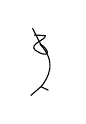
\begin{tikzpicture}[scale=.45]\draw (0,1.1)--(.23,.65)..controls(.58,.4)and(.4,.25)..(.08,.48)..controls(-.12,.65)and(.4,.78)..(.36,.89)--(.05,.91);\draw (.21,.65)..controls(.7,.15)and(.45,-.3)..(.24,-.55)--(-.05,-.8);\draw(.24,-.55)--(.45,-.65);\end{tikzpicture}}

19) \uline{Th. de dualité globale}.
\mspage{35}
\scanpage{37}
\begin{center}- 212 -\end{center}
\hfill n° 391
\[
\begin{split}
\omega_5&=\varepsilon_4+\varepsilon_5+\varepsilon_6+\varepsilon_7+4\varepsilon_8=\\
&=8\alpha_1+12\alpha_2+16\alpha_3+24\alpha_4+20\alpha_5+15\alpha_6+10\alpha_7+5\alpha_8
\end{split}
\]
\[
\begin{split}
\omega_6&=\varepsilon_5+\varepsilon_6+\varepsilon_7+3\varepsilon_8=\\
&=6\alpha_1+9\alpha_2+12\alpha_3+18\alpha_4+15\alpha_5+12\alpha_6+8\alpha_7+4\alpha_8
\end{split}
\]
\[
\begin{split}
\omega_7&=\varepsilon_6+\varepsilon_7+2\varepsilon_8=\\
&=4\alpha_1+6\alpha_2+8\alpha_3+12\alpha_4+10\alpha_5+8\alpha_6+6\alpha_7+3\alpha_8
\end{split}
\]
\[
\omega_8=\varepsilon_7+\varepsilon_8=2\alpha_1+3\alpha_2+4\alpha_3+6\alpha_4+5\alpha_5+4\alpha_6+3\alpha_7+2\alpha_8=\widetilde\alpha.
\]
(VII) On sait que la demi-somme des racines positives est la somme des poids fondamentaux, (§ 6, n° 9, prop. 8), et vaut donc :
\[
\begin{split}
\rho&=\varepsilon_2+2\varepsilon_3+3\varepsilon_4+4\varepsilon_5+5\varepsilon_6+6\varepsilon_7+23\varepsilon_8=\\
&=46\alpha_1+68\alpha_2+91\alpha_3+135\alpha_4+110\alpha_5+84\alpha_6+57\alpha_7+29\alpha_8.
\end{split}
\]
(VIII) On a vu ci-dessus que $\Gamma(R)=\Gamma_{\unsure{o|0}}(R)$ et l'indice de connexion est donc 1.

\figure{\begin{tikzpicture}[scale=.25]\draw (0,.45)--(.35,0)--(.65,.35);\end{tikzpicture}}
(IX) La famille des exposants a 8 termes, et puisque $h=30$, les entiers 1, 7, 11, 13, 17, 19, 23, 29, étrangers à 30, doivent figurer dans cette famille, (§ 8, n° 5, prop. 6) ; ce sont par suite tous les exposants de $W(R)$.

(X) On déduit de (IX) et du § 8, n° 3, cor. 1 de la prop. 3 que l'ordre du groupe de Weyl $W(R)$ est :
\[
2.8.12.14.18.20.24.30=2^{14}.3^5.5^2.7.
\]
(XI) Le même raisonnement qu'au n° 8 montre que le seul automorphisme du schéma de Dynkin $E_8$ est l'identité, les trois chaînes issues du point de ramification ayant des longueurs distinctes.
\mspage{36}
\scanpage{38}
18) Les foncteurs entre cat. \unsure{triangulés|triangulées} \deleted{\unsure{doivent}} commutent au foncteur translation et transforment triangles \unsure{distingués} en \unsure{idem} ....
\[
D(C),\quad D^-(C)\qquad\text{importants }=\text{ sans qu'il y ait des projectifs.}
\]
\[
D^b(C)
\]
\[
Lf^*:D(Y)\longrightarrow D(X)
\]
quand on a $f:X\mathbin{-}Y$ morphisme \uuline{plat} de topos \uline{annelés}
\[
D^+(Y)\mathbin{-}D^+(X)
\]
\[
D^-(Y)\mathbin{-}D^-(X)
\]

$D^+(Y)\mathbin{-}D^+(X)$\qquad définition directe via résolutions injectives

\uline{ou} définition immédiate par ``passage au quotient''

[Pour calculer $Lf^*(K)$, pas la peine de remplacer au préalable $K$ par une résolution injective]

\uuline{NB}. Si $f$ n'est \uline{pas plat}, on \deleted{\unsure{y}} ne peut en général définir raisonnablement
\[
f^*:D^+(Y)\longrightarrow D^+(X)
\]
(de sorte à avoir des bonnes propriétés). Mais dans la suite de ces notes, on explique comment construire raisonnablement $Lf^*:D^-(Y)\mathbin{-}D^-(X)$, \inserted{``dérivé gauche'' de $f^*$,} en utilisant (non pas des rés. projectives mais) des résolutions plates. Ce n'est que si $f$ est à ``Tor-dim. finie'' que \unsure{ça} définit
\[
D^+(Y)\longrightarrow D^+(X)\ ;\quad D^b(Y)\mathbin{-}D^b(X).
\]
\margin{Rien n'empêche de construire un dérivé droit, $Rf^*$, mais il n'a pas le moindre intérêt.}
\mspage{37}
\scanpage{39}
\hfill 40

The results of Chapter I apply. Hence, since $\underline S(X,\underline A)$ is a full subcategory of $\underline P(X,\underline A)$, by I, 3.1, $R_X\circ R_X=R_X$ and by I, 4.12, if $F$ is a sheaf then $R_X(F)=F$. By I, 6.3, $\underline S(X,\underline A)$ is right complete with right roots being $R_X$ applied to the corresponding right root in $\underline P(X,\underline A)$ and if $\underline A$ has a generator, so does $\underline S(X,\underline A)$. Finally, if $\underline A$ is right perfect with a generator, then $\underline S(X,\underline A)$ is abelian, right perfect and has enough injectives.

\figure{\begin{tikzpicture}[scale=.3]\draw (0,0)--(.4,-.03)--(.46,.36);\end{tikzpicture}}
\uline{Proof}:

i) is an immediate consequence of 4.17 and 4.15, Remark ii).

To prove ii) it is sufficient (by 3.1) to construct $R_X(F)$ and $r_F:F\longrightarrow R(\unsure{T|F})$ satisfying the above universal mapping property.

\figure{\begin{tikzpicture}[scale=.35]\draw (0,.03)--(.8,0);\end{tikzpicture}}
Consider $\rho_F:F\longrightarrow P_XF$. By 1.3, $P_XF$ is a sheaf. Let $\{\gamma_i:G_i\longrightarrow P_XF\}$ be the collection of all subsheaves of $P_XF$ through which $\rho_F$ factors; i.e., such that there is a $\delta_i:F\longrightarrow G_i$ with $\gamma_i\unsure{\varepsilon_i|\delta_i}=\rho_F$. Define $R(F)=\bigcap G_i$. Since
\figure{\begin{tikzpicture}[scale=.3]\draw (0,.5)--(.2,0)--(.45,.3);\end{tikzpicture}}
$\underline S(X,\underline A)$ is left closed, and since intersections are left roots (I, § 5, i).) $R(F)$ is a sheaf. Let $\sigma_F:R(F)\longrightarrow P_XF$ be
\mspage{38}
\scanpage{40}
Définition de $R\operatorname{Hom}(F^\cdot,\unsure{G|C}^\cdot)=\operatorname{Hom}^*(F^\cdot,C^\cdot(\unsure{G|C}^\cdot))$
et dans le cas des Modules sur un Topos
\[
R\underline{\operatorname{Hom}}(F^\cdot,\unsure{G|C}^\cdot)
\]
lié au précédent par
\[
\boxed{R\operatorname{Hom}(F^\cdot,\unsure{G|C}^\cdot)=R\Gamma_X R\underline{\operatorname{Hom}}(F^\cdot,\unsure{G|C}^\cdot)}
\]
\[
\left\{\begin{aligned}
\operatorname{Hom}(F^\cdot,\unsure{G|C}^\cdot)&\text{ est aussi noté }\operatorname{Ext}^0(F^\cdot,\unsure{G|C}^\cdot)\\
\operatorname{Hom}(F^\cdot,\unsure{G|C}^\cdot(i))&\simeq\operatorname{Hom}(F^\cdot(-i),\unsure{G|C}^\cdot)\simeq\operatorname{Ext}^i(F^\cdot,\unsure{G|C}^\cdot)
\end{aligned}\right.
\]
Notation $\underline{\operatorname{Ext}}^i(F^\cdot,\unsure{G|C}^\cdot)$ \uline{faisceaux}
\[
\operatorname{Ext}^{p+q}(F^\cdot,\unsure{G|C}^\cdot)\Longleftarrow E_2^{pq}=H^p(X,\underline{\operatorname{Ext}}^q(F^\cdot,\unsure{G|C}^\cdot))
\]
\diagram{\begin{tikzcd}[column sep=0pt,row sep=15pt]
{}'E_2^{pq}=H^p(X,{ } & \operatorname{Ext}^q\arrow[dr,no head,bend right=15] & (F^*\arrow[d,no head] & ,\unsure{G|C}^*)\arrow[dl,no head] & )\\
&&\text{\unsure{pris} terme à terme}
\end{tikzcd}}
\mspage{39}
\scanpage{41}
\mspage{34}

a) Let $\underline{A}$ be a complete category and let $F$ be a presheaf on $X$ with morphisms $r_{VU}:F(U)\longrightarrow F(V)$ for $V\subset U$. For each $x\in X$, define
\[
F_x=\mathop{\mathrm{dir}\,\lim}_{x\in U\in\underline{T}}F(U)
\]
and let $r_{xU}:F(U)\longrightarrow F_x$ be the induced morphism. $F_x$ is called the \uline{stalk} of $F$ at $x$. Clearly if $\varphi:F\longrightarrow F'$ is a presheaf morphism (i.e., natural transformation) then $\varphi$ induces morphisms $\varphi_x:F_x\longrightarrow F'_x$ for all $x\in X$ such that $r'_{xU}\varphi_U=\varphi_xr_{xU}$ whenever $x\in U$.

b) Let $P_XF$ be the presheaf on $X$ such that for each open set $U$, $P_XF(U)=\prod_{x\in U}F_x$. If $V\subset U$, then $p_{VU}:P_XF(U)\longrightarrow P_XF(V)$ is the unique morphism such that $\widetilde{p}_{xU}=\widetilde{p}_{xV}p_{VU}$ where for $x\in U$, $\widetilde{p}_{xU}:\prod_{x\in U}F_x\longrightarrow F_x$ is the projection morphism. If $\varphi:F\longrightarrow F'$, then $P_X\varphi:P_XF\longrightarrow P_XF'$ is the presheaf morphism such that $(P_X\varphi)_U=\prod_{x\in U}\varphi_x$. By definition of $\prod_{x\in U}\varphi_x$, whenever $x\in U$, $\varphi_x\circ\widetilde{p}_{xU}=\widetilde{p}'_{xU}\circ(P_X\varphi)_U$. It is immediate that $P_X:\underline{P}(X,\underline{A})\longrightarrow\underline{P}(X,\underline{A})$ is a functor.
\mspage{40}
\scanpage{42}
Définition des $R_!f_*(F^\cdot)$, ($f$ \uline{compactifiable}).

\diagram{\begin{tikzcd}
X\arrow[r,hook,no head]\arrow[d,"f"',no head]&\overline{X}\arrow[dl,"\overline{f}"]\\
Y&
\end{tikzcd}}
\[
R_!f_*:D^+(X)-D^+(Y)
\]
\[
H^i(R_!f_*)=R^i_!f_*
\]
Reformulation des propriétés \unsure{connues} :

(i) $R_!(gf)_*=(R_!g_*)(R_!f_*)$

si $f,g$ sont deux morphismes compactifiables composables

(ii) Compatibilité aux extensions de la base.

\uline{Remarque} En fait si \deleted{$f$ est à fibres de dim bornée,}\inserted{$Y$ est quasi compact,} on peut définir
\[
R_!f_*:D(X)-D(Y)
\]
induisant
\[
D^-(X)\longrightarrow D^-(Y),\quad D^+(X)\longrightarrow D^+(Y)
\]
\[
D^b(X)-D^b(Y)
\]
\unsure{Ceci|Car} résulte du fait que $f_*$, si $f$ propre à fibres de dim bornée, est \deleted{$\unsure{cd}$}\inserted{de dim} finie.
\mspage{41}
\scanpage{43}
\mspage{38}
and hence such that $p_{U_iU}f=f_i$. Any other $f':X\longrightarrow P_XF(U)$ satisfying $p_{U_iU}f'=f_i$ also satisfies $p_{xU}f'=f_x$ and hence $f'=f$. Thus $P_XF(U)$ satisfies the universal mapping property defining $\mathrm{inv}\,\lim P_XF(U_i)$. Therefore $P_XF$ is a sheaf.

ii) To show that
\[
\operatorname{Hom}_{\underline{S}(X,\underline{A})}(P_XF,P_XF')=\prod_{x\in U}\operatorname{Hom}_{\underline{A}}(F_x,F'_x)
\]
there is obviously a map from the right hand side to the left hand side; namely, if $\{\widetilde{\varphi}_x:F_x\longrightarrow F'_x\}$, define $\varphi:P_XF\longrightarrow P_XF'$ by $\varphi_U=\prod_{x\in U}\widetilde{\varphi}_x$. Conversely, given $\varphi:P_XF\longrightarrow P_XF'$, $\varphi_x:(P_XF)_x\longrightarrow(P_XF')_x$ and hence $\widetilde{\varphi}_x=\widetilde{p}'_x\circ\varphi_x\circ(\rho_F)_x:F_x\longrightarrow F'_x$. It is easily checked that these maps are inverses.

iii) If $F\in\underline{S}(X,\underline{A})$, then by 1.2, $\rho_F:F\longrightarrow P_XF$ is a monomorphism. If $\varphi$ and $\psi:F\longrightarrow F'$ satisfy $P_X\varphi=P_X\psi$, then $(\rho_{F'})\circ\varphi=P_X\varphi\circ\rho_F=P_X\psi\circ\rho_F=(\rho_{F'})\circ\psi$ and, since $\rho_{F'}$ is a monomorphism, $\varphi=\psi$. Hence $P_X$ is a local monomorphism.

iv) To show that $P_X$ is left exact, let
\[
0\longrightarrow F'\longrightarrow F\longrightarrow F''\longrightarrow0
\]
be an exact sequence in $\underline{P}(X,\underline{A})$. Then, by right perfection,
\mspage{42}
\scanpage{44}
Ici, prenant les top. étales sur les préschémas, et les faisceaux \unsure{cts} $A_X$ $(\mathbf{Z}/n\mathbf{Z}=A)$, tous les morphismes de topoi annelés envisagés sont plats.

\figure{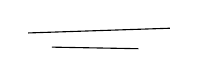
\begin{tikzpicture}\draw (0,0)--(1.8,.06);\draw (.3,-.18)--(1.4,-.2);\end{tikzpicture}}

\diagram{\begin{tikzcd}
\unsure{F}&\\[-15pt]
X\arrow[d,"f"',no head]&X'\arrow[l,"h"']\arrow[d,"f'"]\\
Y&Y'\arrow[l,"g"']
\end{tikzcd}}
Si $f$ quelconque, on définit pour $F^\cdot\in\operatorname{Ob}D^+(X)$ un hom (dans la catégorie dérivée $D^+(Y')$)
\[
(*)\qquad \deleted{Rf'_*(h^*F^\cdot)\longleftarrow}\boxed{g^*(Rf_*(F^\cdot))\longrightarrow Rf'_*(h^*(F^\cdot))}.
\]
Passant aux faisceaux de \unsure{coh.}, cela redonne
\[
(*_i)\qquad g^*R^if_*(F))\longrightarrow R^if'_*(h^*(F)))
\]
\uline{Lorsque} $f$ \uline{est propre} ce sont des isom, puisque on sait que les $(*_i)$ le sont.
\mspage{43}
\scanpage{45}
\mspage{39}
\[
0\longrightarrow F'_x\longrightarrow F_x\longrightarrow F''_x\longrightarrow0
\]
is exact for all $x\in X$. Since $\prod$ preserves kernels (I, 4.7)
\[
0\longrightarrow P_XF'\longrightarrow P_XF\longrightarrow P_XF''
\]
is exact in $\underline{P}(X,\underline{A})$.

1.4 \uline{Theorem}:

i) $\underline{S}(X,\underline{A})$ is a left closed subcategory of $\underline{P}(X,\underline{A})$ and hence, if $\underline{A}$ is left complete, then so is $\underline{S}(X,\underline{A})$.

ii) Let $\underline{A}$ be complete (I, 4.1) and have enough small objects (I, 5.2). Then $\underline{S}(X,\underline{A})$ is a right reflective subcategory of $\underline{P}(X,\underline{A})$, with reflection $R_X$.

iii) If $\underline{A}$ is right perfect then $R_X$ is exact.

\uline{Remarks}: In \unsure{other} words, if $F$ is a presheaf on $X$ with values in $\underline{A}$, then there is an associated sheaf $R_X(F)$ together with a morphism $r_F:F\longrightarrow R_X(F)$ such that if $\varphi:F\longrightarrow G$ is any presheaf morphism with $G$ a sheaf, then there is a unique
\[
\varphi':R_X(F)\longrightarrow G
\]
with $\varphi=\varphi'r_F$.
\diagram{\begin{tikzcd}
F\arrow[r,"r_F"]\arrow[dr,"\varphi"']&R_X(F)\arrow[d,"\varphi'"]\\
&G
\end{tikzcd}}
\mspage{44}
\scanpage{46}
\deleted{\unsure{\S}} 19) \uline{Le th de dualité globale} : énoncé
\figure{\begin{tikzpicture}[scale=.25]\draw (0,-.45)..controls(-.07,.05)and(-.02,.4)..(.25,.28);\end{tikzpicture}}
général pour un morphisme lisse compactifiable
\mspage{45}
\scanpage{47}
\mspage{46}
\deleted{
- \mspage{IV-1007} -

plication b)$\Rightarrow$c)\inserted{sans hypothèse de séparation}. Nous ignorons s'il en est encore ainsi (sans hypothèse de séparation) pour $n$ quelconque. Rappelons que, sans hypothèse de séparation, l'implication c)$\Rightarrow$b) n'est plus valable\inserted{même pour $n=1$} (0,15.1.12 (iii)).

\uline{19.6. Suites régulières relativement à un module \deleted{quotient}\inserted{filtré}}.

(19.6.1) Soient $A$ un anneau, $\underline{f}=(f_1,\ldots,f_n)$ une suite\inserted{finie} d'éléments de $A$, $\underline{J}=f_1A+\ldots+f_nA$ l'idéal qu'elle engendre, et considérons une suite exacte de $A$-modules
\diagram{\begin{tikzcd}
0\arrow[r]&R\arrow[r,"j"]&N\arrow[r,"p"]&M\arrow[r]&0
\end{tikzcd}}
où l'on suppose que $N$ est muni d'une filtration décroissante $(N_k)$ formée de sous-$A$-modules, avec $N_0=N$. On pose $R_k=R\cap N_k$ (filtration induite par $(N_k)$), $M_k=p(N_k)$ (filtration quotient de $(N_k)$), et on désigne par $\operatorname{gr}_\bullet(N)$, $\operatorname{gr}_\bullet(R)$ et $\operatorname{gr}_\bullet(M)$ les $A$-modules gradués associés à ces trois filtrations. On pose d'autre part pour tout $k$,
\[
N'_k=N_k+\underline{J}N_{k-1}+\ldots+\underline{J}^{k-1}N_1+\underline{J}^kN_0
\]
de sorte que \deleted{$\unsure{M'_k=p(N'_k)}$} $M'_k=p(N'_k)=M_k+\underline{J}M_{k-1}+\ldots+\underline{J}^{k-1}M_1+\underline{J}^kM_0$ ; on pose d'autre part $R'_k=R\cap N'_k$ (filtration \uline{induite} par $(N'_k)$), et on note \deleted{\unsure{par}} $\operatorname{gr}'_\bullet(N)$, $\operatorname{gr}'_\bullet(M)$ et $\operatorname{gr}'_\bullet(R)$ les $A$-modules gradués associés à ces trois filtrations ; on a donc un diagramme commutatif de suites exactes

(19.6.1.1)
\diagram{\begin{tikzcd}[column sep=small]
0\arrow[r]&\operatorname{gr}_\bullet(R)\arrow[r,"\operatorname{gr}(j)"]\arrow[d]&\operatorname{gr}_\bullet(N)\arrow[r,"\operatorname{gr}(p)"]\arrow[d]&\operatorname{gr}_\bullet(M)\arrow[r]\arrow[d]&0\\
0\arrow[r]&\operatorname{gr}'_\bullet(R)\arrow[r,"\operatorname{gr}'(j)"']&\operatorname{gr}'_\bullet(N)\arrow[r,"\operatorname{gr}'(p)"']&\operatorname{gr}'_\bullet(M)\arrow[r]&0
\end{tikzcd}}
\inserted{où les flèches verticales sont les homomorphismes canoniques d'un module gradué associé à une filtration dans le module gradué associé à une filtration moins forte.}

On notera que si l'on pose
\[
R''_k=R_k+\underline{J}R_{k-1}+\ldots+\underline{J}^{k-1}R_1+\underline{J}^kR_0
\]
on a évidemment $R''_k\subset R'_k$, mais les filtrations $(R''_k)$ et $(R'_k)$ sont en général distinctes ; on notera $\operatorname{gr}''_\bullet(R)$ le $A$-module gradué associé à la filtration $(R''_k)$.

(19.6.2) On a défini en (\uline{0},15.1.5.2) les homomorphismes surjectifs gradués de degré 0
\[
\psi_N:(\operatorname{gr}_\bullet(N)\otimes_A(A/\underline{J}))[T_1,\ldots,T_n]\longrightarrow\operatorname{gr}'_\bullet(N)
\]
}
\figure{\begin{tikzpicture}[x=.32cm,y=.32cm]
\draw (2.7,8.7) .. controls (2.1,9) and (4.4,15.9) .. (7.6,19.7);
\draw (3.8,2.7) .. controls (4.5,2.6) and (10.1,17.3) .. (12.5,19.7);
\draw (7.5,2.2) .. controls (8.4,.8) and (10.7,9.3) .. (16.5,12.7);
\draw (1.5,16.5) .. controls (1.9,17) and (2.7,17.1) .. (2.5,17.3);
\end{tikzpicture}}
\scanpage{48}
20) \uline{Exemple} \deleted{$\unsure{S=\operatorname{Spec}k}$} avec un corps de base, sép clos p.ex.
\[
H^i_!(X,F)^\vee\simeq H^{-i}(X,DF)
\]
Si $F$ loc. ct.
\[
H^i_!(X,F)^\vee\simeq H^{2d-i}(X,\underline{\operatorname{Hom}}(F,\mu_{nX}^{\otimes d}))
\]
On retrouve le th. de finitude de Artin.

Si $S$ quelconque, on \unsure{trouve} si les $R^i_!f_*(F)$ sont loc constants (p.ex. $f$ propre lisse!)
\[
\operatorname{Hom}(R^i_!f_*(F),(\mathbf{Z}/n\mathbf{Z})_X)\simeq R^{-i}_{\deleted{!}}f_*(D(F))
\]
(ce qui implique que les $R^{-i}_!f_*(DF)$ sont loc constants) et plus spécialement, si $F$ est loc. constant
\[
\operatorname{Hom}(R^i_!f_*(F),(\mathbf{Z}/n\mathbf{Z})_X)\simeq R^{2d-i}_{\deleted{!}}f_*(\operatorname{Hom}(F,\mu_{nX}^{\otimes d})
\]
Donc dans ces cas, on dispose de la \deleted{finitude}\inserted{constructibilité} des $R^{\deleted{\unsure{2d-i}}}f_{\deleted{!}}\deleted{\operatorname{Hom}}G$ $(G=DF\ldots)$

On peut généraliser en supposant que l'hypothèse n'est satisfaite que pour $i\leq i_0$, la conclusion le sera pour $j\geq2d-i_0\ldots$
\mspage{47}
\scanpage{49}
- 211 - \hfill n\textsuperscript{o} 391

(III) En vertu du § 8, n\textsuperscript{o} 3, formule (4), on a $h=n/\ell=30$.

(IV) La plus grande racine pour l'ordre opposé de l'ordre lexicographique sur $\mathrm{R}^8$ est évidemment $\varepsilon_7+\varepsilon_8=2\alpha_1+3\alpha_2+4\alpha_3+6\alpha_4+5\alpha_5+4\alpha_6+3\alpha_7+2\alpha_8$ ; c'est la plus grande racine $\widetilde\alpha$, (§ 6, n\textsuperscript{o} 6, cor. 2 de la prop. 13), et on vérifie que son ordre est $h-1=29$. Elle est orthogonale à toutes les racines simples sauf $\alpha_8$, et l'on a $(\widetilde\alpha|\alpha_8)=-1$.

(V) Les \uline{coracines} s'obtiennent en remplaçant les $\varepsilon_i$ par les $\varepsilon_i^*$ dans les expressions des racines de $R$, et $R^*$ est donc isomorphe à $R$. Comme toutes les racines sont de même longueur, la \uline{forme bilinéaire canonique} pour $R$ est $(x|y)/2h=(x|y)/60$ et la longueur des racines est $1/\sqrt{30}$, (§ 8, n\textsuperscript{o} 5, \uline{Remarque}). Le nombre des racines non orthogonales à une racine donnée est $4h-6=114$ et le nombre $\gamma$ est égal à $h^2=900$.

(VI) Comme $\Gamma_{\unsure{o|0}}(R^*)$ est le réseau $L_3(V^*)$, son associé dans $V=\mathrm{R}^4$ est $L_3(V)$, (n\textsuperscript{o} 4), c'est-à-dire $\Gamma_{\unsure{o|0}}(R)$, autrement dit, on a $\Gamma(R)=\Gamma_{\unsure{o|0}}(R)$. Le calcul des poids fondamentaux, formant \unsure{le|la} base duale de $(\alpha_i^*)$, donne :
\[
\omega_1=2\varepsilon_8=4\alpha_1+5\alpha_2+7\alpha_3+10\alpha_4+8\alpha_5+6\alpha_6+4\alpha_7+2\alpha_8
\]
\[
\begin{aligned}
\omega_2&=\frac12(\varepsilon_1+\varepsilon_2+\varepsilon_3+\varepsilon_4+\varepsilon_5+\varepsilon_6+\varepsilon_7+5\varepsilon_8)=\\
&=5\alpha_1+8\alpha_2+10\alpha_3+15\alpha_4+12\alpha_5+9\alpha_6+6\alpha_7+3\alpha_8
\end{aligned}
\]
\[
\begin{aligned}
\omega_3&=\frac12(-\varepsilon_1+\varepsilon_2+\varepsilon_3+\varepsilon_4+\varepsilon_5+\varepsilon_6+\varepsilon_7+7\varepsilon_8)=\\
&=7\alpha_1+10\alpha_2+14\alpha_3+20\alpha_4+16\alpha_5+12\alpha_6+8\alpha_7+4\alpha_8
\end{aligned}
\]
\[
\begin{aligned}
\omega_4&=\varepsilon_3+\varepsilon_4+\varepsilon_5+\varepsilon_6+\varepsilon_7+5\varepsilon_8=\\
&=10\alpha_1+15\alpha_2+20\alpha_3+30\alpha_4+24\alpha_5+18\alpha_6+12\alpha_7+6\alpha_8
\end{aligned}
\]
\mspage{48}
